%% For Slides
\documentclass[xcolor=x11names,compress,mathserif]{beamer}
%% For handouts
%\documentclass[xcolor=x11names,compress,mathserif,12pt,handout]{beamer}
%% To put multiple pages (say 2x3) per page in pdf,  use command 
%% pdfnup --a4paper --keepinfo --nup 2x3 --frame true \
%%      --scale 0.95 --no-landscape --outfile handout.pdf <input>.pdf
%% End of For Handout

\usepackage{etex}
%% Beamer Layout %%%%%%%%%%%%%%%%%%%%%%%%%%%%%%%%%%
\useoutertheme[subsection=false,shadow]{miniframes}
\useinnertheme{default}
\usefonttheme{structureitalicserif}
\usepackage{palatino}
%% packages from the paper
\usepackage{schemepgm}
\usepackage{graphicx}
\usepackage{mathrsfs}
\usepackage{graphpap}
\usepackage{tabularx}
\usepackage{epsfig}
\usepackage{pstricks}
\usepackage{pst-text}
\usepackage{pst-node}
\usepackage{pst-tree}
\usepackage{pst-coil}
\usepackage{pst-rel-points}
\usepackage{boxedminipage}
\usepackage{algorithmic}
\usepackage{amssymb}
\usepackage{amsmath}
\usepackage{calc}
%%%%%%%%%% IMPERATIVE %%%%%%%%%%%%

%%%%%%%%%%%%%%%%%%%%%%%%%%%%%%%%%%%%%%%%%%%%%%%%%%%%%%%%%%%%%%%%%%
%%% Comment out a part of latex document
\newcommand{\cmt}[1]{}
\newcommand{\akadd}[1]{\protect{\red  #1}}
\newcommand{\akdel}[1]{\protect{\blue #1}}
\newcommand{\del}[1]{\protect{\magenta #1}}

\newcommand{\mybox}{\hfill\ensuremath{\Diamond}}
\newcommand{\NDIn}[1]{\mbox{\sf In$_#1$}}
\newcommand{\NDOut}[1]{\mbox{\sf Out$_#1$}}
%\newcommand{\x}{\cx}
%\newcommand{\y}{\cy}
%%%%%%%%%%%%%%%%%%%%%%%%%%%%%%%%%%%%%%%%%%%%%%%%%%%%%%%%%%%%%%%%%%

%%%%%%%%%%%%%%%%%%%%%%%%%%%%%%%%%%%%%%%%%%%%%%%%%%%%%%%%%%%%%%%%%%
%%%% Programs in latex 
\protect{\newlength{\FTABL}}
\protect{\newlength{\TABL}}
\protect{\newlength{\BRACE}}
\settowidth{\BRACE}{\{}

%%%%%%%%%%%%%%%%%%%%%%%%%%%%%%%%%%%%%%%%%%%%%%%%%%%%%%%%%%%%%%%%%%

 \newcommand{\ntbar}{\ensuremath{\overline\nt}}
%% %%%%%%%%%%%%%%%%%%%%%%%%%%%%%%%%%%%%%%%%%%%%%%%%%%%%%%%%%%%%%%%%%%
%%% Special pictures
\newcommand{\myarrow}{\mbox{%
 \psset{unit=1cm}%
 \begin{pspicture}(0,0)(.27,.2)%
  \psline[linewidth=.15mm]%
  (0,.1)(.125,.1)(.125,.035)(.25,.1)(.125,.165)(.125,.1)%
  \end{pspicture}}%
} 



%%
%% paths and derefs
\newcommand{\epath}{\mathsf{ep}}
\newcommand{\paths}{{\sf paths}}
\newcommand{\dpaths}{{\sf dpaths}}
\newcommand{\Pf}[2]{\ensuremath{\Pfonly_{\!\!#1}^{\,#2}}}
\newcommand{\Pfonly}{\ensuremath{\mathsf{PF}}}
\newcommand{\Pp}[2]{\ensuremath{\Pponly_{\!\!#1}^{\,#2}}}
\newcommand{\Pponly}{\ensuremath{\mathsf{PP}}}
\newcommand{\Pe}[3]{\ensuremath{\Peonly(#1, #2, #3)}}
\newcommand{\Peonly}{\ensuremath{\mathsf{PE}}}
\newcommand{\Peb}[3]{\ensuremath{\Pebonly(#1, #2, #3)}}
\newcommand{\Pebonly}{\ensuremath{\Peonly!}}
\newcommand{\Pv}{\ensuremath{\mathsf{P}}}
\newcommand{\Pvphi}{\ensuremath{\Pv^\emptyset}}
\newcommand{\Ddf}[2]{\ensuremath{\Ddfonly_{\!\!#1}^{\,#2}}}
\newcommand{\Ddfonly}{\ensuremath{\mathsf{DF}}}
\newcommand{\Dp}[2]{\ensuremath{\Dponly_{\!\!#1}^{\,#2}}}
\newcommand{\Dponly}{\ensuremath{\mathsf{DP}}}
\newcommand{\De}[3]{\ensuremath{\Deonly(#1, #2, #3)}}
\newcommand{\Deonly}{\ensuremath{\mathsf{DE}}}
%%\newcommand{\Deb}[3]{\ensuremath{\Debonly(#1, #2, #3)}}
%%\newcommand{\Debonly}{\ensuremath{\Deonly!}}
\newcommand{\Dv}{\ensuremath{\mathsf{D}}}
\newcommand{\Dvphi}{\ensuremath{\Dv^\emptyset}}
\newcommand{\derefs}{{\sf derefs}}

\newcommand{\bw}[1]{\ensuremath{\overline{#1}}} % backward
\newcommand{\cat}[2]{\ensuremath{#1#2}} % concat
\newcommand{\expshare}{\ensuremath{\mathsf{ExpS}}} % generic path

%% heap location and heap cell
\newcommand{\loc}[1]{\ensuremath{\mbox{\sf Loc}[{#1}]}}
\newcommand{\cell}[1]{\ensuremath{\mbox{\sf Cell}[{#1}]}}

%% type of labels
\newcommand{\acar}{\ensuremath{\mathbf{0}}}
\newcommand{\acdr}{\ensuremath{\mathbf{1}}}
\newcommand{\bcar}{\ensuremath{\bar\acar}}
\newcommand{\bcdr}{\ensuremath{\bar\acdr}}
\newcommand{\clazy}{\ensuremath{{\mathbf{2}}}}
\newcommand{\bX}  {\ensuremath{\bar{X}}}
\newcommand{\acarset}{\ensuremath{\lbrace\acar\rbrace}}
\newcommand{\acdrset}{\ensuremath{\lbrace\acdr\rbrace}}
\newcommand{\bcarset}{\ensuremath{\lbrace\bcar\rbrace}}
\newcommand{\bcdrset}{\ensuremath{\lbrace\bcdr\rbrace}}
\newcommand{\epsilonset}{\ensuremath{\lbrace\epsilon\rbrace}}

%%  transfer eqns - alias
\newcommand{\Af}[2]{\ensuremath{\Afonly_{#1}^{\,#2}}}
\newcommand{\Afonly}{\ensuremath{\mathsf{SF}}}
\newcommand{\Ap}[2]{\ensuremath{\Aponly_{#1}^{\,#2}}}
\newcommand{\Aponly}{\ensuremath{\mathsf{SP}}}
\newcommand{\Ae}[3]{\ensuremath{\Aeonly(#1, #2, #3)}}
\newcommand{\Aeonly}{\ensuremath{\mathsf{SE}}}
\newcommand{\Aa}[2]{\ensuremath{\Aaonly(#1, #2)}}
\newcommand{\Aaonly}{\ensuremath{\mathsf{SS}}}
\newcommand{\Av}{\ensuremath{\mathsf{S}}}
\newcommand{\Aphi}{\ensuremath{\Av^\emptyset}}
\newcommand{\Dfonly}{\ensuremath{\mathsf{D}}}
\newcommand{\Ufonly}{\ensuremath{\mathsf{I}}}
%\newcommand{\calls}[2]{\ensuremath{{\mathit{\!c}_{{\mathit #1}_#2}}}}
\newcommand{\calls}[2]{\ensuremath{{\mathit{\!c}_{{\mathit #1}}^#2}}}
%%\newcommand{\calls}[2]{\ensuremath{{\overline{\mathit #1}_{#2}}}}
%%  transfer eqns - liveness
\newcommand{\Uf}[2]{\ensuremath{\mathsf{I}_{\mathit #1}^{#2}}}
\newcommand{\Lfun}[3]{\ensuremath{\mathcal{L}(#1,#2,#3)}}
\newcommand{\Lfunonly}{\ensuremath{\mathcal{L}}}

\newcommand{\Df}[2]{\ensuremath{\mathsf{D}_{\mathit #1}^{#2}}}


\newcommand{\Lf}[3]{\ensuremath{\Lfonly_{\mathit #1}^{#2}( {\mathit #3})}}
\newcommand{\Lfonly}{\ensuremath{\mathsf{LF}}}
\newcommand{\Lfone}[1]{\ensuremath{\Lfonly_{\mathit #1}}}
\newcommand{\Le}[1]{\ensuremath{\Leonly({\mathit #1})}}
\newcommand{\Leonly}{\ensuremath{\mathsf{LE}}}
\newcommand{\Lp}[2]{\ensuremath{\Lponly_{#1}^{\,#2}}}
\newcommand{\Lponly}{\ensuremath{\mathsf{LP}}}
\newcommand{\Ld}[3]{\ensuremath{\Ldonly_{\mathit #1}^{#2}( {\mathit #3})}}
\newcommand{\Ldonly}{\ensuremath{\mathsf{LD}}}
\newcommand{\Lvc}[2]{\ensuremath{\Lv_{\mathit #1}^{\mathit #2}}}

\newcommand{\Lv}{\ensuremath{\mathsf{L}}}
\newcommand{\Lvphi}{\ensuremath{\Lv^\emptyset}}
\newcommand{\Leb}[3]{\ensuremath{\Lebonly(#1, #2, #3)}}
\newcommand{\Lebonly}{\ensuremath{\Leonly!}}
\newcommand{\NFA}{\mbox{\sf nfa}}
\newcommand{\lang}[1]{\ensuremath{\mathscr{L}({#1})}}
\newcommand{\Lan}[1]{\ensuremath{\Lv_{{#1}}}}
\newcommand{\Lanv}[2]{\ensuremath{\Lv_{{#1}}^{#2}}}
\newcommand{\dfa}[2]{\ensuremath{\mathsf{dfa}_{{#1}}^{#2}}}
%%  transfer eqns - availability
\newcommand{\AVf}[2]{\ensuremath{\AVfonly_{#1}^{\,#2}}}
\newcommand{\AVfonly}{\ensuremath{\mathsf{AvF}\,}}
\newcommand{\AVp}[2]{\ensuremath{\AVponly_{#1}^{\,#2}}}
\newcommand{\AVponly}{\ensuremath{\mathsf{AvP}\,}}
\newcommand{\AVgp}[2]{\ensuremath{\AVgponly_{#1}^{\,#2}}}
\newcommand{\AVgponly}{\ensuremath{{\mathsf{AvBP}}}}
\newcommand{\AVgf}[2]{\ensuremath{\AVgfonly_{#1}^{\,#2}}}
\newcommand{\AVgfonly}{\ensuremath{{\mathsf{AvBF}\,}}}
\newcommand{\AVe}[3]{\ensuremath{\AVeonly(#1, #2, #3)}}
\newcommand{\AVeonly}{\ensuremath{\mathsf{AvE}\,}}
\newcommand{\AVv}{\ensuremath{\mathsf{AV}}}
%\newtheorem{observation}[theorem]{Observation}

%%  transfer eqns - anticipability
\newcommand{\ANf}[2]{\ensuremath{\ANfonly_{#1}^{\,#2}}}
\newcommand{\ANfonly}{\ensuremath{\mathsf{AnF}}}
\newcommand{\ANp}[2]{\ensuremath{\ANponly_{#1}^{\,#2}}}
\newcommand{\ANponly}{\ensuremath{\mathsf{AnP}}}
\newcommand{\ANgp}[2]{\ensuremath{\ANgponly_{#1}^{\,#2}}}
\newcommand{\ANgponly}{\ensuremath{{\mathsf{AnBP}}}}
\newcommand{\ANgf}[2]{\ensuremath{\ANgfonly_{#1}^{\,#2}}}
\newcommand{\ANgfonly}{\ensuremath{{\mathsf{AnBF}}}}
\newcommand{\ANe}[3]{\ensuremath{\ANeonly(#1, #2, #3)}}
\newcommand{\ANeonly}{\ensuremath{\mathsf{AnE}}}
\newcommand{\ANv}{\ensuremath{\mathsf{AN}}}
\newcommand{\ANvphi}{\ensuremath{\ANv^\emptyset}}
\newcommand{\mmap}[3]{\ensuremath{\mathcal{M}_{\mathit{#1}}(\mathit{#2})(\mathit{#3})}}
\newcommand{\pmap}[1]{\ensuremath{\mathcal{P}_{\mathit{#1}}}}
\newcommand{\deltacall}[3]{\delta_{#1}({#2},{#3})}
%% union?
\newcommand{\plus}{$\cup$}

%% -> arrows, =def
\newcommand{\rightk}[1]{\ensuremath{\stackrel{\scriptstyle #1}{\rightarrow}}}
\newcommand{\rightstar}{\rightk{\star}}
%\newcommand{\eqdef}{\ensuremath{\stackrel{\scriptstyle def}{=}}}
\newcommand{\eqdef}{\ensuremath{=}}

%% functions

\newcommand{\listc}{\mbox{\tt l}}
\newcommand{\lista}{\mbox{\tt l1}}
\newcommand{\listb}{\mbox{\tt l2}}

%% nfa and cfg
\newcommand{\nfa}{\ensuremath{\mathbf{N}}}
\newcommand{\nfabar}{\ensuremath{\overline\nfa}}

\newcommand{\start}{{\sf init}}
\newcommand{\prim}{\ensuremath{P}}
\newcommand{\exit}{{\sf pgm}}
\newcommand{\gram}{\ensuremath{G}}
\newcommand{\nt}{\ensuremath{N}}
\newcommand{\var}[1]{\ensuremath{\langle #1\rangle}}

\newcommand{\TwoCells}[2]{%
\psset{unit=.25mm}
\begin{pspicture}(0,-2)(36,18)
\psframe(0,-5)(36,15)
\psline(18,-4)(18,15)
\putnode{zarb1342}{origin}{9}{5}{\rnode{#1}{}}
\putnode{zarb0102}{origin}{27}{5}{\rnode{#2}{}}
\end{pspicture}%
}

\newcommand{\TwoCellNull}[2]{%
\psset{unit=.25mm}
\begin{pspicture}(0,-2)(36,18)
\psframe(0,-5)(36,15)
\psline(18,-4)(18,15)
\psline(18,-4)(36,15)
\putnode{z}{origin}{9}{5}{\rnode{#1}{}}
\putnode{z}{origin}{27}{5}{\rnode{#2}{}}
\end{pspicture}%
}

\newcommand{\TwoCellsD}[2]{%
\psset{unit=.25mm}
\begin{pspicture}(0,-2)(36,18)
\psframe(0,-5)(36,15)
\psline(18,-4)(18,15)
\putnode{z}{origin}{9}{5}{\rnode{#1}{}}
\putnode{z}{origin}{27}{5}{\rnode{#2}{}}
\putnode{z}{origin}{9}{5}{%
      \psframebox[linestyle=none,fillstyle=hlines,hatchsep=2,framesep=8,
      hatchcolor=blue]{}}
\end{pspicture}%
}
\newcommand{\TwoCellsA}[2]{%
\psset{unit=.25mm}
\begin{pspicture}(0,-2)(36,18)
\psframe(0,-5)(36,15)
\psline(18,-4)(18,15)
\putnode{z}{origin}{9}{5}{\rnode{#1}{}}
\putnode{z}{origin}{9}{5}{%
   \psframebox[linestyle=none,fillstyle=hlines,hatchsep=2,framesep=8,
   hatchcolor=blue]{}}
\putnode{z}{origin}{27}{5}{\rnode{#2}{}}
\end{pspicture}%
}
\newcommand{\TwoCellsAD}[2]{%
\psset{unit=.25mm}
\begin{pspicture}(-6,-2)(42,18)
%\psframe(0,-5)(36,15)
%\psline(18,-4)(18,15)
\putnode{z}{origin}{9}{5}{\rnode{#1}{}}
\putnode{z}{origin}{9}{5}{%
   \psframebox[linestyle=none,fillstyle=solid,framesep=8,
   fillcolor=lightgray]{}}
\putnode{z}{origin}{27}{5}{%
      \psframebox[linestyle=none,fillstyle=solid,framesep=8,
   fillcolor=lightgray]{}}
\psccurve[fillstyle=solid,fillcolor=lightgray,linecolor=black]
(0,-5)(-6,5)(0,15)(12,20)(24, 15)(30,17)(36,15)(42,5)(36,-5)(24, -10)(12, -5)(6, -8)
\end{pspicture}%
}
% meta scheme command
\newcommand{\MIF}{\mbox{$\mathsf{if}$}}
\newcommand{\MEQ}{\mbox{$\mathsf{eq?}$}}
\newcommand{\MLET}{\mbox{$\mathsf{let}$}}
\newcommand{\MIN}{\mbox{$\mathsf{in}$}} 
%\newcommand{\IF}{\mbox{$\mathsf{if}$}}
%\newcommand{\SLET}{\mbox{$\mathsf{let}$}}
%\newcommand{\SIN}{\mbox{$\mathsf{in}$}} 

% others..
\newcommand{\candidates}[1]{\ensuremath{\mbox{\sf Candidates}(#1)}}
\newcommand{\scvars}[1]{\ensuremath{\mathsf{ScopeVars}(#1)}}
\newcommand{\expvars}[1]{\ensuremath{\mathsf{FV}(#1)}}
\newcommand{\mainpgm}{\ensuremath{\mathbf{main}}}
\newcommand{\main}{\ensuremath{\mathbf{main}}}
\newcommand{\updateenv}[3]{{\sf update(#1, #2, #3)}}
\newcommand{\pair}[2]{(#1, #2)}

\newcommand{\pia}{\ensuremath{\pi_{a}}}
\newcommand{\pib}{\ensuremath{\pi_{b}}}


\newenvironment{minieqnarray}
{\begin{minipage}{\textwidth}\begin{eqnarray}}
{\end{eqnarray}\end{minipage}}

%%% EFFECTIVENESS OF GC 
\newcommand{\deltarch}{\mbox{%
 \ensuremath{\delta_{\mbox{\footnotesize\sf rch}}}}}
\newcommand{\deltagc}{\mbox{%
 \ensuremath{\delta_{\mbox{\footnotesize\sf gc}}}}}
\newcommand{\GCstructure}{{\tt GC\_structure}}
\newcommand{\GCflag}{{\tt GC\_flag}}
\newcommand{\CreateTime}{{\tt Create\_time}}
\newcommand{\UseTime}{{\tt Use\_time}}
\newcommand{\CollTime}{{\tt Collection\_time}}
\newcommand{\exectime}{\mbox{\sf  T}}

\newcommand{\manual}[1]{{\protect#1}}

%% Benchmark names
\newcommand{\silex}{\mbox{\tt silex}}
\newcommand{\lalr}{\mbox{\tt lalr}}
\newcommand{\eopl}{\mbox{\tt eopl}}
\newcommand{\prolog}{\mbox{\tt prolog}}
\newcommand{\sudoku}{\mbox{\tt sudoku}}
\newcommand{\cipher}{\mbox{\tt cipher}}

%% helpful definitions
%%\renewcommand{\citeNP}{\cite}
\newcommand{\figtwo}{figure*}
\newcommand{\capsize}{}
\newcommand{\figrule}{}
\newcommand{\figtworule}{}

%% scheme program vars/constants
%% \renewcommand{\px}{\mbox{$\mathbf{x}$}}
%% \renewcommand{\py}{\mbox{$\mathbf{y}$}}
%% \renewcommand{\pz}{\mbox{$\mathbf{z}$}}
%% \renewcommand{\pw}{\mbox{$\mathbf{w}$}}
%% \newcommand{\pthree}{\mbox{$\mathbf{3}$}}
%% \newcommand{\pfour}{\mbox{$\mathbf{4}$}}
%% \newcommand{\pfive}{\mbox{$\mathbf{5}$}}
%% \newcommand{\psix}{\mbox{$\mathbf{6}$}}
%% \newcommand{\ptwo}{\mbox{$\mathbf{2}$}}
%% \newcommand{\append}{\mbox{$\mathbf{append}$}}
%% \newcommand{\set}{\mbox{$\mathbf{set{\mbox{\rm \bf !}}}$}}
%% \newcommand{\setcar}{\mbox{$\mathbf{set{\mbox{\rm \bf -}}car{\mbox{\rm \bf !}}}$}}
%% \newcommand{\setcdr}{\mbox{$\mathbf{set{\mbox{\rm \bf -}}cdr{\mbox{\rm \bf !}}}$}}

%% other defs
\newcommand{\nullifiable}{\mbox{\sf Nullifiable}}
\newcommand{\properprefix}{\mbox{\sf ProperPrefix}}
\newcommand{\prefix}{\mbox{\sf  Prefix}}
\newcommand{\linknull}{{\sf LinkNullify}}
\newcommand{\pathnullify}{{\sf PathNullify}}
\newcommand{\nullins}{{\sf GenNullCode}}
\newcommand{\nullstatements}{\mbox{\sf null-statements}}
\newcommand{\isnull}{\mbox{\sf isnull}}
\newcommand{\mymark}{\mbox{\sf Mark}}
\newcommand{\sbegin}{\mbox{\sf BEGIN}}
\newcommand{\map}{\mbox{\sf map}}
\newcommand{\nullset}{\ensuremath{\mathsf{N}}}
\newcommand{\insnull}[2]{\mbox{$\mathsf{InsertNull(#1,#2)}$}}  
\newcommand{\insnullfn}{\mbox{$\mathsf{InsertNull}$}}   

\newcommand{\compnullfn}{\mbox{$\mathsf{Nullify}$}} 
\newcommand{\compnull}[2]{\compnullfn(#1, #2)}
\newcommand{\compnullpgm}[1]{\mbox{$\mathsf{Nullifypgm(#1)}$}}
\newcommand{\compnulldef}[1]{\mbox{$\mathsf{Nullifydef(#1)}$}}

\newcommand{\zz}{{\sf z}}
\newcommand{\yy}{{\sf y}}
\newcommand{\xx}{{\sf x}}
\newcommand{\ww}{{\sf w}}
\newcommand{\uu}{{\sf u}}
\newcommand{\aap}{{\sf a}}
\newcommand{\result}{{\sf result}}

%% \newtheorem{lemma}{Lemma}[section]
%% \newtheorem{example}{Example}[section]
%% \newtheorem{theorem}{Theorem}[section]
%% \newtheorem{definition}{Definition}[section]
%% \newtheorem{corollary}{Corollary}[section]
%% \newtheorem{property}{Property}[section]
%% \newcommand{\qed}{\hfill\nobreak \ifvmode \relax \else
%%   \ifdim\lastskip<1.5em \hskip-\lastskip
%%   \hskip1.5em plus0em minus0.5em \fi \nobreak
%%   \vrule height0.75em width0.5em depth0.25em\  fi}
\newcommand{\qed}{\hfill\ensuremath{\square}}
 \newenvironment{proof}[1][Proof]{\begin{trivlist}
 \item[\hskip \labelsep {\bfseries #1}]}{\hfill\qed\end{trivlist}}

\newcommand{\expr}[1]{\ensuremath{#1}}
%\newcommand{\pv}[1] {\mbox{\tt #1}}
\newcommand{\db}[1]{{\bf [\![}#1{\bf ]\!]}}
\newcommand{\nat}{I\!\!N}
\newcommand{\lenprime}{\ \vdash^{l'}\ }
\newcommand{\len}{\ \vdash^l\ }
\newcommand{\sen}{\ \vdash^s\ }
\newcommand{\fen}{\ \vdash^f\ }
\newcommand{\den}{\ \vdash^f\ }
\newcommand{\argsen}{\ \vdash^{args}\ }
\newcommand{\pen}{\ \vdash^p\ }
\newcommand{\fsen}{\ \vdash^{fs}\ }
\newcommand{\psen}{\ \vdash^{ps}\ }

\newcommand{\last}{\mbox{last}}
\newcommand{\rightmost}{\mbox{rightmost}}
\newcommand{\before}{\mbox{before}}
\newcommand{\befen}{\ \vdash^{\sf before}}
\newcommand{\lasten}{\ \vdash^{\sf last}}
\newcommand{\rmen}{\ \vdash^{\sf rightmost}}
\newcommand{\rhos}{\ensuremath{\red \rho_s}}
\newcommand{\pgmpt}[1]{\ensuremath{\red \pi_{#1}}}
\newcommand{\multireduct}{\ensuremath{\stackrel{+}{\longrightarrow}}}
\newcommand{\avrightarrow}{\ensuremath{\longrightarrow}}
\newcommand{\multireductav}{\ensuremath{\stackrel{+}{\avrightarrow}}}
\newcommand{\heap}{\ensuremath{H}}       % heap
\newcommand{\ppn}[2]{\ensuremath{#2}} % prog point
\newcommand{\pp}[2]{\ensuremath{#2}} % prog point
\newcommand{\lvintp}{\ensuremath{\zeta}}
\newcommand{\avintp}{\lvintp}
\newcommand{\locs}{\mbox{\tt locs}} 
\newcommand{\llv}{\ensuremath{\mathcal{L}}}
\newcommand{\aav}{\ensuremath{\mathcal{A}}}
\newcommand{\aan}{\ensuremath{\mathcal{N}}}
\newcommand{\gl}{\mbox{\em G}}




%% packages from the paper
\setbeamerfont{title like}{shape=\scshape}
\setbeamerfont{frametitle}{shape=\scshape}

\setbeamercolor*{lower separation line head}{bg=DeepSkyBlue4} 
\setbeamercolor*{normal text}{fg=black,bg=white} 
\setbeamercolor*{alerted text}{fg=red} 
\setbeamercolor*{example text}{fg=black} 
\setbeamercolor*{structure}{fg=black} 
 
\setbeamercolor*{palette tertiary}{fg=black,bg=black!10} 
\setbeamercolor*{palette quaternary}{fg=black,bg=black!10} 

\newcommand{\cmt}[1]{}
\renewcommand{\(}{\begin{columns}}
\renewcommand{\)}{\end{columns}}
\newcommand{\<}[1]{\begin{column}{#1}}
\renewcommand{\>}{\end{column}}

%%%%%%%%%%%%%%%%%%%%%%%%%%%%%%%%%%%%%%%%%%%%%%%%%%
\begin{document}
%%%%%%%%%%%%%%%%%%%%%%%%%%%%%%%%%%%%%%%%%%%%%%%%%%%%%%
%%%%%%%%%%%%%%%%%%%%%%%%%%%%%%%%%%%%%%%%%%%%%%%%%%%%%%
\section{\scshape Motivation}
\begin{frame}
\title{Liveness-Based Garbage Collection for Lazy Languages}
\author{
        {\bf Prasanna Kumar, Amitabha Sanyal}\\{\it Indian Institute of
          Technology, Bombay}\\ \and
       {\bf Amey Karkare}\\{\it Indian Institute of Technology, Kanpur}
}

%% \date{
%% 	%% \begin{tikzpicture}[decoration=Koch curve type 2] 
%% 	%% 	\draw[DeepSkyBlue4] decorate{ decorate{ decorate{ (0,0) -- (3,0)}}}; 
%% 	%% \end{tikzpicture}  
%% 	%% \\
%% 	June 14th, 2016
%% }
\date{\today}
\titlepage
\end{frame}

%%%%%%%%%%%%%%%%%%%%%%%%%%%%%%%%%%%%%%%%%%%%%%%%%%%%%%
%%%%%%%%%%%%%%%%%%%%%%%%%%%%%%%%%%%%%%%%%%%%%%%%%%%%%%
%% \begin{frame}{Outline of Talk}
%% \tableofcontents
%% \end{frame}

%%%%%%%%%%%%%%%%%%%%%%%%%%%%%%%%%%%%%%%%%%%%%%%%%%%%%%
%%%%%%%%%%%%%%%%%%%%%%%%%%%%%%%%%%%%%%%%%%%%%%%%%%%%%%

\begin{frame}{Liveness based GC}
    \begin{itemize}\itemsep0.75em
    \item Current garbage collectors retain heap allocated data
      that  is {\em  reachable}.
    \item Programs need only data that will be used in future.
      Such data is said to be {\em live}.
    \item Our idea: 
      \begin{itemize}
      \item We do  a liveness analysis of {\em heap  data} and provide
        GC with its result.
      \item Modify GC to mark data for retention {\em only if it is live}.
      \end{itemize}
    \item Consequences:
      \begin{itemize}
      \item  Fewer cells  marked.  \pause More  garbage collected  per
        collection. \pause Fewer garbage collections. \pause
      \item Programs expected to run faster and with smaller heap.
      \end{itemize}
    \end{itemize}
\end{frame}

%%%%%%%%%%%%%%%%%%%%%%%%%%%%%%%%%%%%%%%%%%%%%%%%%%%%%%
%%%%%%%%%%%%%%%%%%%%%%%%%%%%%%%%%%%%%%%%%%%%%%%%%%%%%%
\begin{frame}{An Example}
%%%%%%%%%%%%%%%%%%%%%%%%%%%%%%%%%%%%%%%%%%%%%%%%%%%%%%%%%%%%%%%%%%%%%%%%%%%
%%% MOTIVATING EXAMPLE
  %
%%%%%%%%%%%%%%%%%%%%%%%%%%%%%%%%%%%%%%%%%%%%%%%%%%%%%%%%%%%%%%%%%%%%%%%%%%%
%%% MOTIVATING EXAMPLE
%% \newcommand{\nilfigure}
%% {\scalebox{0.75}{
%% \psset{unit=1mm,nodesep=0mm,labelsep=0.5mm}
%% \begin{pspicture}(0,0)(1,1)
%% %\psgrid[xunit=1cm,yunit=1cm,gridwidth=.2pt,subgridwidth=.1pt,subgriddiv=5,subgridcolor=gray,gridcolor=blue](0,0)(1,1)
%% \putnode{start}{origin}{0}{0}{}
%% \putnode{stop}{origin}{10}{10}{}
%% \ncline[offsetB=0,nodesepB=0,linewidth=.7]{-}{start}{stop} %here
%% \end{pspicture}
%% }}

%\begin{columns}
 % \begin{column}{0.5\textwidth}
%\begin{boxedminipage}{\textwidth}{
    \scalebox{0.75}{\sf
      \renewcommand{\arraystretch}{1}{
	\begin{uprogram}
	  \UFL\ \hspace*{-.31\TAL} (\DEFINE\ (\plength\  \lista)
	  \UNL{1}  (\SIF~(\NULLQ \ \lista)
	  0
	  \UNL{2}      ($+$\ 1\ (\plength\ (\CDR\  \lista)))))
          \UNL{2}
          \UNL{0}\ \hspace*{-.31\TAL} (\DEFINE\ (\pfun\  \listb)
	  \UNL{1}  ($+$\ 1\ (\CAR\  \listb)))
          %         \UNL{2}\;\;\;\;\;
          \UNL{0}
	  \UNL{0} \hspace*{-.49\TAL} $\pi_\mainpgm$ : (\LET\ \pz\   $\leftarrow$(\CONS\ ($+$\ $4$ $5$)\
          \UNL{0} \;\;\;\;\;\;\;\;\;\;\;\;\;\;\;\;\;\;\;\;\;\;\; (\CONS\ ($+$\ $5$ $2$) \NIL)) \IN
	  \UNL{0} \;\;\;\;\;\;\;\;\;\;\;\;(\SIF\ $*$\ 
	  \UNL{1} \;\;\;\;\;\;\;\;\;\;\;\; $\pi_1$: (\plength\ \pz\ )
	  \UNL{1} \;\;\;\;\;\;\;\;\;\;\;\; $\pi_2$: (\pfun\ \pz\ )))
	\end{uprogram}
  }}
%\end{boxedminipage}
  %% \end{column}
  %% \begin{column}{0.5\textwidth}
  %%   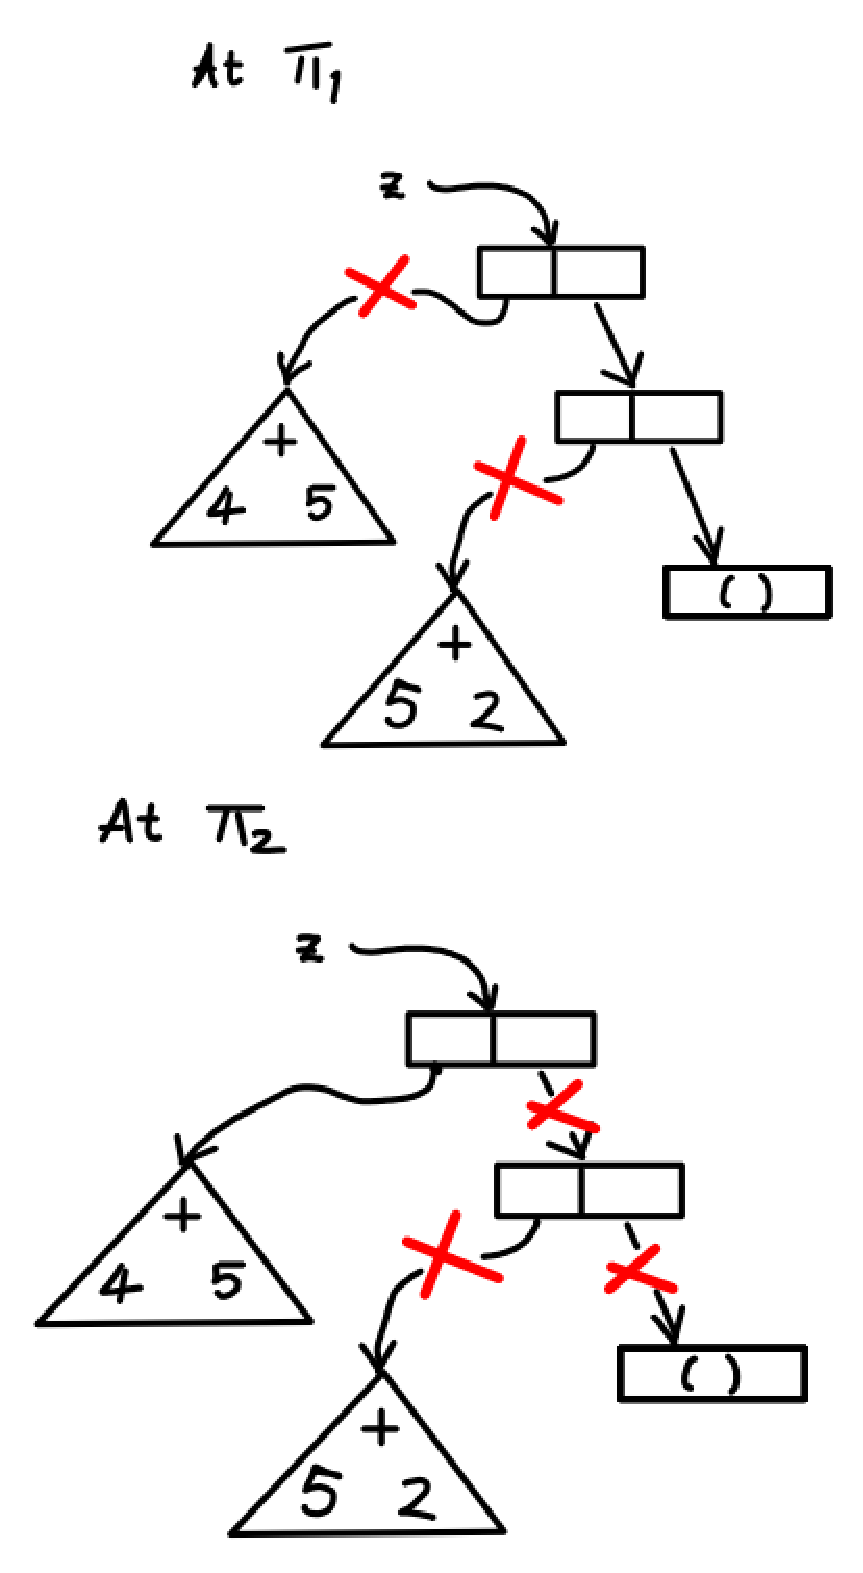
\epsfig{file=mem-graph.eps, height=6.5cm}
  %% \end{column}
%\end{columns}


  \begin{columns}
    \begin{column}{0.5\textwidth}
      \begin{boxedminipage}{\textwidth}
        {\scalebox{0.75}{\sf
	\renewcommand{\arraystretch}{1}{
	  \begin{uprogram}
            \UNL{0} \hspace*{-.49\TAL} $\pi_\mainpgm$ : (\LET\ \pz\   $\leftarrow$(\CONS\ ($+$\ $4$ $5$)\
            \UNL{0} \;\;\;\;\;\;\;\;\;\;\;\;\;\;\;\;\;\;\;\;\;\;\; (\CONS\ ($+$\ $5$ $2$) \NIL)) \IN
	    \UNL{0} \;\;\;\;\;\;\;\;\;\;\;\;(\SIF\ $*$\ 
	    \UNL{1} \;\;\;\;\;\;\;\;\;\;\;\; $\pi_1$: (\plength\ \pz\ )
	    \UNL{1} \;\;\;\;\;\;\;\;\;\;\;\; $\pi_2$: (\pfun\ \pz\ )))
       	  \end{uprogram}
        }}}
      \end{boxedminipage}
    \end{column}
    \begin{column}{0.5\textwidth}
      %    Add diagram for liveness of $\pz$ at $\pi_1$  and $\pi_2$
      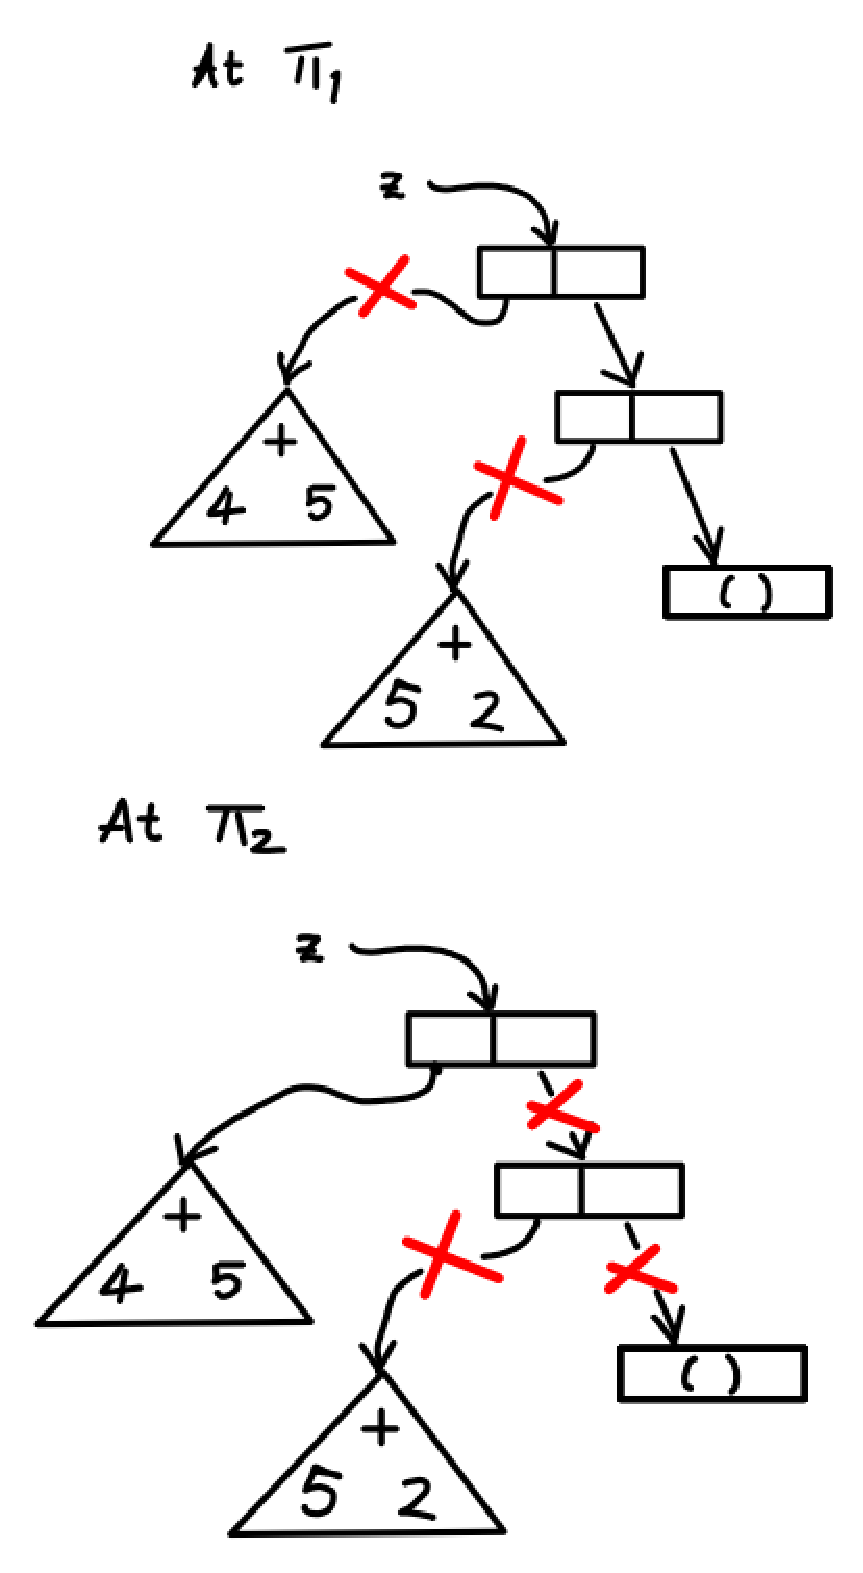
\epsfig{file=mem-graph.eps, height=6.5cm}
    \end{column}
  \end{columns}
    
\bigskip
\begin{itemize}
\item<1->{\em  Expression $(+\ 5\ 2)$ never gets evaluated and $(+\ 4\ 5)$ gets evaluated only if $*$ is false.}  
\end{itemize}
\end{frame}

%%%%%%%%%%%%%%%%%%%%%%%%%%%%%%%%%%%%%%%%%%%%%%%%%%%%%%
%% \begin{frame} {Lazy evaluation}
%% \begin{itemize}
%% \item An evaluation  strategy in which evaluation of  an expression is
%%   postponed until its value is needed
%%   \begin{itemize}
%%   \item Binding  of a  variable to  an expression  {\bf does  not force
%%     evaluation} of the expression
%%   \end{itemize}
%% \item Every expression is evaluated at most once
%% \end{itemize}
%% \end{frame}
%%%%%%%%%%%%%%%%%%%%%%%%%%%%%%%%%%%%%%%%%%%%%%%%%%%%%%
\section{\scshape Our method}
%%%%%%%%%%%%%%%%%%%%%%%%%%%%%%%%%%%%%%%%%%%%%%%%%%%%%%
\begin{frame}{The language analyzed}
\begin{columns}
  \begin{column}[T]{0.45\textwidth}
\small
    \begin{itemize} \itemsep0.75em
    \item First order Scheme-like lazy functional language.
    \item In Administrative Normal Form (ANF).
%    \item The order  of
%      evaluation of function arguments is made explicit.
    \end{itemize}
\normalsize
  \end{column}
  \begin{column}[T]{0.55\textwidth}
    
\small
\begin{eqnarray*}
   p \in \mathit{Prog} & ::= & d_1 \ldots d_n \,\, e_\mainpgm \\
    d \in Fdef & ::= & (\DEFINE\,\, (f\,\, 
    x_1 \,\, \ldots \,\, x_n)\,\,
    e) 
    \hspace{1.7em} \mbox{} \\
e \in \mathit{Expr} & ::= &
\left\{\begin{array}{lll}
       (\SIF\,\, x\,\, e_1\,\, e_2) && \mbox{} \\  
       (\LET\,\, x \leftarrow a\,\, \IN\,\, e) && \mbox{} \\
       (\RETURN\,\, x) && \mbox{}
    \end{array}\right. \\
a \in \mathit{App} & ::= &
\left\{\begin{array}{lrl}
       k && \mbox{}\\
       (\CONS\,\, {\red x_1}\,\, {\red x_2}) && \mbox{} \\ 
       (\CAR\,\, {\red x)} &  (\CDR\,\, {\red x)} & \mbox{} \\ 
       (\NULLQ\,\, {\red x}) & (\PRIM\,\, {\red x_1}\,\, {\red x_2}) & \mbox{} \\ 
%        (\NULLQ\,\, x) && \mbox{\em ---  tester} \\ 
%       (\ID\,\, x) && \mbox{\em ---  identity function (for inlining)} \\ 
%        (\PRIM\,\, x_1\,\, x_2) && \mbox{\em --- generic arithmetic} \\ 
       \multicolumn{2}{l}{(f\,\,{\red  x_1}\,\,\ldots\,\, {\red x_n})} 
            & \mbox{} 
    \end{array}\right.
\end{eqnarray*}



  \end{column}
\end{columns}
\end{frame}
%%%%%%%%%%%%%%%%%%%%%%%%%%%%%%%%%%%%%%%%%%%%%%%%%%%%%%
%% \begin{frame}{The language analyzed}
%%   
%%%%%%%%%%%%%%%%%%%%%%%%%%%%%%%%%%%%%%%%%%%%%%%%%%%%%%%%%%%%%%%%%%%%%%%%%%%
%%% MOTIVATING EXAMPLE
%% \newcommand{\nilfigure}
%% {\scalebox{0.75}{
%% \psset{unit=1mm,nodesep=0mm,labelsep=0.5mm}
%% \begin{pspicture}(0,0)(1,1)
%% %\psgrid[xunit=1cm,yunit=1cm,gridwidth=.2pt,subgridwidth=.1pt,subgriddiv=5,subgridcolor=gray,gridcolor=blue](0,0)(1,1)
%% \putnode{start}{origin}{0}{0}{}
%% \putnode{stop}{origin}{10}{10}{}
%% \ncline[offsetB=0,nodesepB=0,linewidth=.7]{-}{start}{stop} %here
%% \end{pspicture}
%% }}

%\begin{columns}
 % \begin{column}{0.5\textwidth}
%\begin{boxedminipage}{\textwidth}{
    \scalebox{0.75}{\sf
      \renewcommand{\arraystretch}{1}{
	\begin{uprogram}
	  \UFL\ \hspace*{-.31\TAL} (\DEFINE\ (\plength\  \lista)
	  \UNL{1}  (\SIF~(\NULLQ \ \lista)
	  0
	  \UNL{2}      ($+$\ 1\ (\plength\ (\CDR\  \lista)))))
          \UNL{2}
          \UNL{0}\ \hspace*{-.31\TAL} (\DEFINE\ (\pfun\  \listb)
	  \UNL{1}  ($+$\ 1\ (\CAR\  \listb)))
          %         \UNL{2}\;\;\;\;\;
          \UNL{0}
	  \UNL{0} \hspace*{-.49\TAL} $\pi_\mainpgm$ : (\LET\ \pz\   $\leftarrow$(\CONS\ ($+$\ $4$ $5$)\
          \UNL{0} \;\;\;\;\;\;\;\;\;\;\;\;\;\;\;\;\;\;\;\;\;\;\; (\CONS\ ($+$\ $5$ $2$) \NIL)) \IN
	  \UNL{0} \;\;\;\;\;\;\;\;\;\;\;\;(\SIF\ $*$\ 
	  \UNL{1} \;\;\;\;\;\;\;\;\;\;\;\; $\pi_1$: (\plength\ \pz\ )
	  \UNL{1} \;\;\;\;\;\;\;\;\;\;\;\; $\pi_2$: (\pfun\ \pz\ )))
	\end{uprogram}
  }}
%\end{boxedminipage}
  %% \end{column}
  %% \begin{column}{0.5\textwidth}
  %%   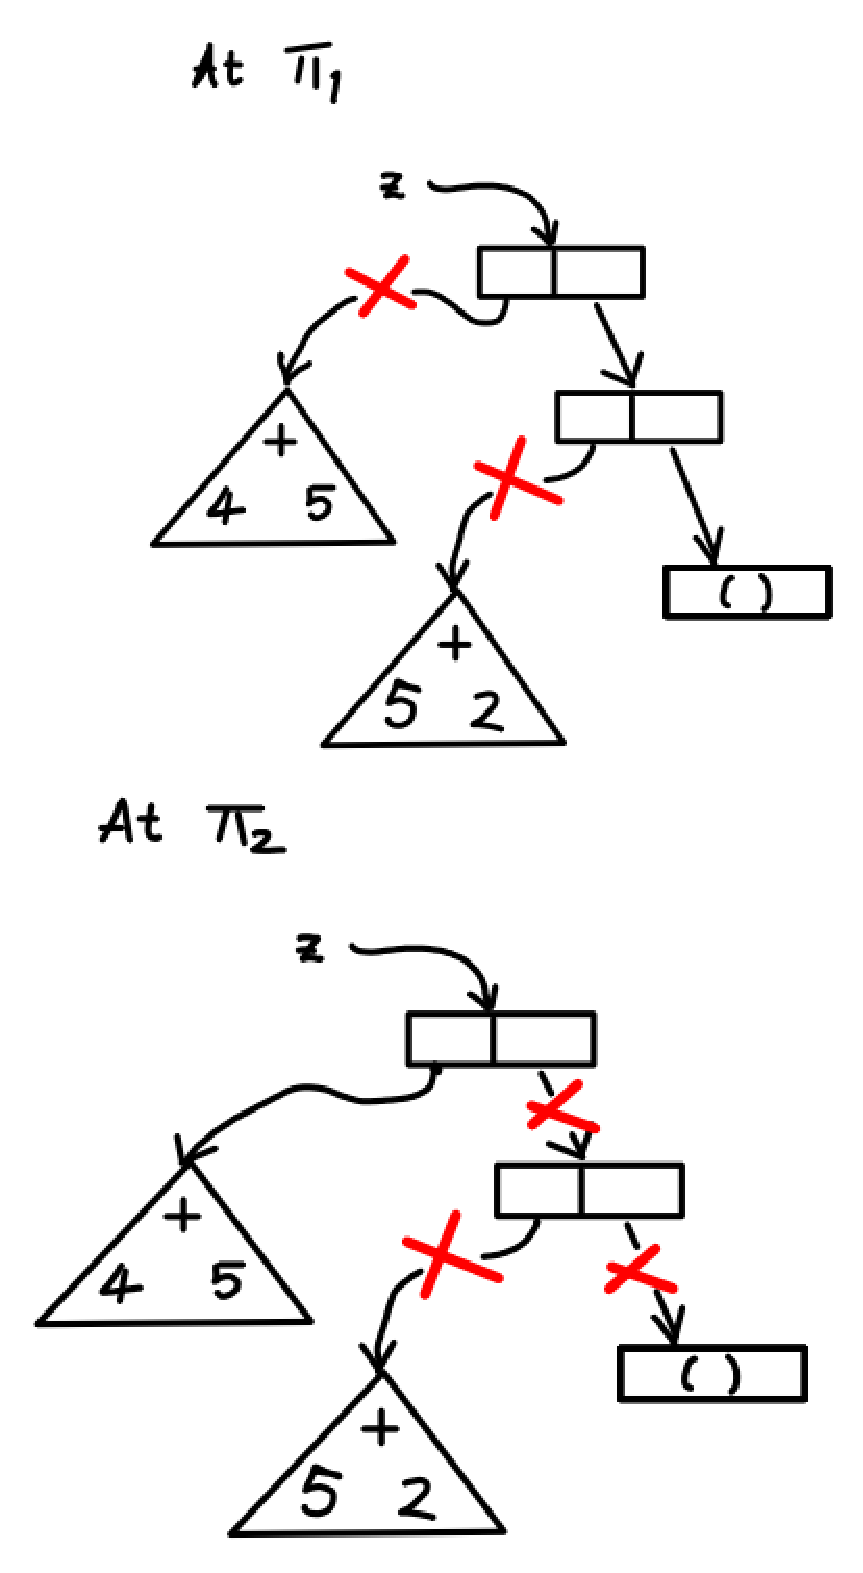
\epsfig{file=mem-graph.eps, height=6.5cm}
  %% \end{column}
%\end{columns}


%% \end{frame}
\section{\scshape LGC for lazy languages}
%%%%%%%%%%%%%%%%%%%%%%%%%%%%%%%%%%%%%%%%%%%%%%%%%%%%%%
\begin{frame}{Basic Concepts and Notations--Demand}
  \begin{center}
     (\CAR\ (\CDR\ \pw)) \\
  \end{center}
  \pause
\centerline{

%%%%%%%%%%%%%%%%%%%%%%%%%%%%%%%%%%%%%%%%%%%%%%%%%%%%%%%%%%%%%%%%%%%%%%%%%%%
%%% MOTIVATING EXAMPLE
\newcommand{\nilfigure}
{\scalebox{0.75}{
\psset{unit=1mm,nodesep=0mm,labelsep=0.5mm}
\begin{pspicture}(0,0)(1,1)
%\psgrid[xunit=1cm,yunit=1cm,gridwidth=.2pt,subgridwidth=.1pt,subgriddiv=5,subgridcolor=gray,gridcolor=blue](0,0)(1,1)
\putnode{start}{origin}{0}{0}{}
\putnode{stop}{origin}{10}{10}{}
\ncline[offsetB=0,nodesepB=0,linewidth=.7]{-}{start}{stop} %here
\end{pspicture}
}}

 %%%%%%%%%%%%%%%%%%%%%%%%%%%%%%%%%%%%%%%%%%%%%%%%%%%%%%%%%%%%%%%%%%%%%%%%%%%
 %%% MOTIVATING EXAMPLE


       \raisebox{-25mm}{\scalebox{.65}{
         %%%%%%%%%%%%%%%%%%%%%Uday's stuff%%%%%%%%%%%%%%%%%%%%%%%%%
       \psset{unit=1mm}
       \psset{linewidth=.3mm}
       \begin{pspicture}(0,-5)(70,60)
% \psgrid[xunit=1cm,yunit=1cm,gridwidth=.2pt,subgridwidth=.1pt,subgriddiv=5,subgridcolor=gray,gridcolor=blue](0,-5)(7,6)
         %\psframe(0,0)(73,60)
         %%%%%%%%%%%%%%%%%%%%%%%%%%%%%%%%%%%%%%%%%%%%%%%%%%%%%%%%%%%%%%%%
         \putnode{o}{origin}{13}{50}{}%{\TwoCells{o1}{o2}}
         \putnode{a}{o}{-10}{-15}{\psframebox{3}}
%         \putnode{r}{origin}{26}{38}{}
%         \ncline[offsetB=-.5,nodesepB=.1]{*->}{o1}{a}
%         \putnode{b}{o}{0}{-3}{\psframebox[linestyle=none,framesep=.5]{\scalebox{.63}{\nilfigure}}}
 %	\ncline[offsetB=-.5,nodesepB=.1]{*->}{o2}{b}
         %\ncline[offsetB=-.5,nodesepB=.1]{->}{o2}{b}
%         \putnode{y}{o}{-14}{8}{\psframebox[linestyle=none,framesep=.5]{y}}
%        {\nccurve[nodesepB=-.2,angleA=330,angleB=120]{->}{y}{o}}
%         \aput[-3.5](.5){\scalebox{1.2}{\psframebox[framesep=.2,linestyle=none,fillstyle=solid,
%                   fillcolor=white]{$\times$}}}
         %%%%%%%%%%%%%%%%%%%%%%%%%%%%%%%%%%%%%%%%%%%%%%%%%%%%%%
         \putnode{c}{o}{25}{0}{\TwoCells{c1}{c2}}
         \putnode{d}{c}{10}{-10}{\TwoCells{d1}{d2}}
         \putnode{e}{d}{-13}{-12}{\TwoCells{e1}{e2}}
         \putnode{f}{d}{13}{-12}{\TwoCells{f1}{f2}}
%         \nccurve[nodesepB=-.2,angleA=330,angleB=120,linecolor=red]{->}{r}{e}
         \ncline[nodesepB=-.5]{*->}{c2}{d}
         \ncline[nodesepB=-.5,linewidth=.7]{->}{c2}{d}
         \nccurve[ncurv=1,angleA=180,angleB=0]{*->}{c1}{a}
         \aput[-3.5](.2){\scalebox{1.2}{\psframebox[framesep=.2,linestyle=none,fillstyle=solid,
               fillcolor=white]{$\times$}}}
         \nccurve[nodesepB=-.5,angleA=240,angleB=70,linecolor=red]{*->}{d1}{e}
         \nccurve[nodesepB=-.5,angleA=240,angleB=70,linewidth=.7,linecolor=red]{->}{d1}{e}
         \nccurve[nodesepB=-.5,angleA=300,angleB=110]{*->}{d2}{f}
         \aput[-3.5](.5){\scalebox{1.2}{\psframebox[framesep=.2,linestyle=none,fillstyle=solid,
               fillcolor=white]{$\times$}}}
         \putnode{w}{c}{-8}{8}{\psframebox[linestyle=none,framesep=.2]{w}}
 %        \putnode{ww}{c}{15}{8}{\psframebox[linestyle=none,framesep=.2]{z}}
         \nccurve[nodesepB=-.2,angleA=330,angleB=120,linewidth=.7]{->}{w}{c}
         %%%%%%%%%%%%%%%%%%%%%%%%%%%%%%%%%%%%%%%%%%%%%%%%%%%%%%%%%%%%%%%%%%
         \putnode{g}{e}{-8}{-12}{\psframebox{4}}
         \putnode{h}{e}{8}{-14}{\TwoCells{h1}{h2}}
         \putnode{i}{f}{-8}{-11}{\psframebox{6}}
 %	\putnode{j}{f}{8}{-11}{\psframebox[linestyle=none,framesep=.5]{\NIL}}
         \ncline[offsetB=-.5,nodesepB=.1]{*-}{e1}{e1}
         \ncline[linestyle=dashed,offsetB=-.5,nodesepB=.1,linewidth=.7]{->}{e1}{g}
         %here
         \putnode{j1}{f}{0}{-3}{\psframebox[linestyle=none,framesep=0]{\scalebox{.63}{\nilfigure}}}
         \putnode{j2}{h}{0}{-3}{\psframebox[linestyle=none,framesep=.5]{\scalebox{.63}{\nilfigure}}}

 %        \aput[-3.2](.6){\scalebox{1.2}{\psframebox[framesep=.1,linestyle=none,fillstyle=solid,
 %	      fillcolor=white]{$\times$}}} %and here
         \ncline[offsetB=-.5,nodesepB=-.3]{*-}{e2}{e2}
         \ncline[linestyle=dashed,offsetB=-.5,nodesepB=.1,linewidth=.7]{->}{e2}{h} 
 %	\aput[-3.2](.5){\scalebox{1.2}{\psframebox[framesep=.1,linestyle=none,fillstyle=solid,
 %	      fillcolor=white]{$\times$}}} %and here

         \ncline[offsetB=-.5,nodesepB=.1]{*->}{f1}{i}
         \ncline[offsetB=-.5,nodesepB=.1]{*->}{f2}{j}
         \nccurve[nodesepB=-.2,angleA=270,angleB=90]{->}{ww}{d}
         \aput[-3.2](.55){\scalebox{1.2}{\psframebox[framesep=.1,linestyle=none,fillstyle=solid,
               fillcolor=white]{$\times$}}}
         %%%%%%%%%%%%%%%%%%%%%%%%%%%%%%%%%%%%%%%%%%%%%%%%%%%%%%%%%%%%%%%%%%
         \putnode{k}{h}{-8}{-11}{\psframebox{5}}
 %	\putnode{l}{h}{8}{-11}{\psframebox[linestyle=none,framesep=.5]{\NIL}}
         \ncline[offsetB=-.5,nodesepB=.1]{*-}{h1}{h1}
         \ncline[linestyle=dashed,offsetB=-.5,nodesepB=.1,linewidth=.7]{->}{h1}{k}
 %	\ncline[offsetB=-.5,nodesepB=.1]{*->}{h2}{l}
         %%%%%%%%%%%%%%%%%%%%%%%%%%%%%%%%%%%%%%%%%%%%%%%%%%%%%%%%%%%%%%%%%%
       \end{pspicture}}} 


}
  \begin{itemize}
  \item Demand  (notation: $\sigma$) is a description  of intended use
    of the result of an expression.
  \end{itemize}
\end{frame}

%%%%%%%%%%%%%%%%%%%%%%%%%%%%%%%%%%%%%%%%%%%%%%%%%%%%%%
%%%%%%%%%%%%%%%%%%%%%%%%%%%%%%%%%%%%%%%%%%%%%%%%%%%%%%
\section{\scshape Liveness}
\begin{frame}{Basic Concepts and Notations--Liveness }
\small
\begin{columns}
  \begin{column}[T]{0.75\textwidth}
    \begin{itemize}\itemsep0.75em
    \item {\em Access paths:} Strings over \{\acar, \acdr\}.
      
      \hspace*{.25cm}   \acar\  -- access \CAR\ field \\
      \hspace*{.25cm}   \acdr\  -- access \CDR\ field 
    \item Denote traversals over the heap graph
    \item {\em Liveness environment:} 
      \only<1>
          {Maps root variables    to set of access paths.
            \begin{eqnarray*}
              \Lanv{i}{}&:&
              \left\{\begin{array}{l}
              y \mapsto \emptyset\\
              z \mapsto \{\epsilon\}\\
              w \mapsto \{\epsilon, 1, 10, 100\}
              \end{array}\right.
            \end{eqnarray*}
          }
          \only<2>
              {Alternate representation.
                \begin{eqnarray*}
                  \Lanv{i}{}&:&
                  \left\{\begin{array}{l}
                  \emptyset \;\; \cup  \\
                  \{z.\epsilon\} \;\; \cup\\
                  \{w.\epsilon, w.1, w.10, w.100\}
                  \end{array}\right.
                \end{eqnarray*} 
              }
    \end{itemize}
  \end{column}
  \begin{column}[T]{0.25\textwidth}
    \fbox{\centerline{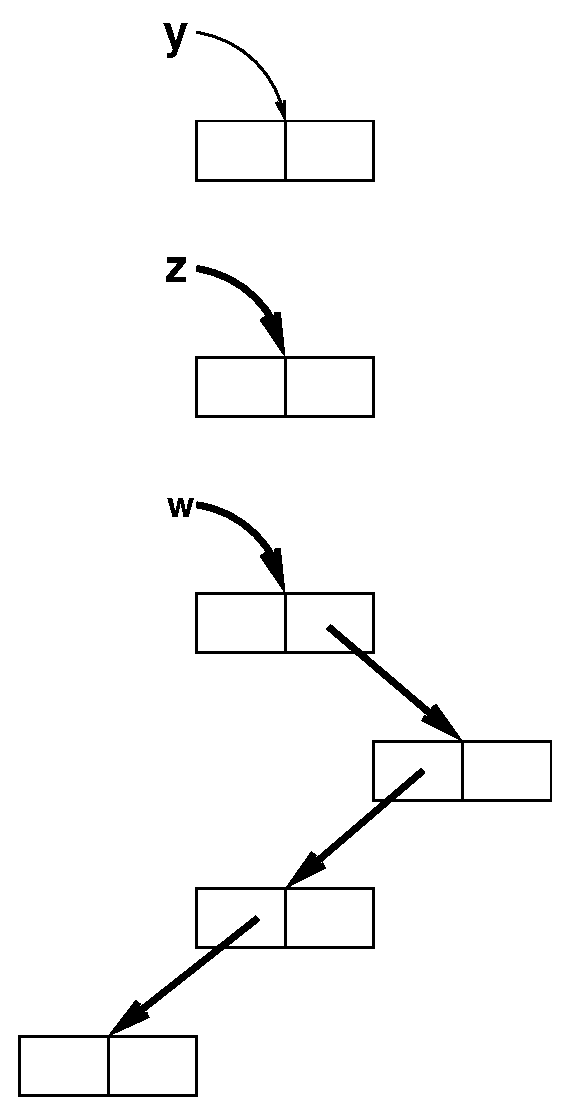
\epsfig{file=example-liveness-environment.eps, height=5cm}}}
  \end{column}
\end{columns}

\bigskip
\bigskip

\onslide<1>{Notation: We write \Lanv{i}{}(\px) as  \normalsize\Lanv{i}{\px}}
\end{frame}

%%%%%%%%%%%%%%%%%%%%%%%%%%%%%%%%%%%%%%%%%%%%%%%%%%%%%%

%%%%%%%%%%%%%%%%%%%%%%%%%%%%%%%%%%%%%%%%%%%%%%%%%%%%%%
\begin{frame}{Liveness analysis}
  \begin{itemize}
  \item {\bf  GOAL:} Compute  Liveness Environment at  various program
    points, statically. 
  \item Assume that all paths in the result of $\mainpgm$ are live, i.e. demand is $(0 + 1)^*$ or $\sigma_{all}$.
  \item Propagate this demand through the program using liveness rules.
  \end{itemize}
\end{frame}
%%%%%%%%%%%%%%%%%%%%%%%%%%%%%%%%%%%%%%%%%%%%%%%%%%%%%%
\begin{frame}{Liveness analysis}
  \begin{columns}
    \begin{column}[T]{0.5\textwidth}
       \hspace*{-.3cm}\renewcommand{\arraystretch}{1}{
         \begin{uprogram}
           \UNL{1}\hspace*{-.4cm} $\pi_\mainpgm\!\!:\, $(\LET\  \px\  $\leftarrow$ ($\CONS$ ($+$ 5 2) \NIL)  \IN
           \UNL{2}   \hspace*{-.3cm}   $\pi_9\!\!:\, $(\LET\ \pz\ $\leftarrow$ ($\CONS$ ($+$ 4 5 ) \px) \IN
           \UNL{3}   \hspace*{-.3cm}   $\pi_{10}\!\!:\, $(\SIF\ $*$
           \UNL{4}   \hspace*{-.35cm} $\pi_{11}\!\!:\, $(\LET\ \pw\  $\leftarrow$  (\plength\ \pz) \IN
           \UNL{5}   \hspace*{-.38cm}  $\pi_{12}\!\!:\, $(\RETURN\ \pw)
           \UNL{4}   \hspace*{-.35cm}  $\pi_{13}\!\!:\, $(\LET\ \pb\  $\leftarrow$ (\pfun\  \pz) \IN
           \UNL{5}   \hspace*{-.38cm} $\pi_{14}\!\!:\,$(\RETURN\ \pb))))))
       \end{uprogram}}
    \end{column}
    \begin{column}[T]{0.6\textwidth}
      \hspace*{-.8cm}  \renewcommand{\arraystretch}{1}{
        \begin{uprogram}
          \UNL{1} (\DEFINE\ (\plength~\lista)
          
          \UNL{2}  $\pi_1\!\!:\, $(\LET\ \xtest\ $\leftarrow $\ (\NULLQ~\lista) \IN
          

          \UNL{3}     $\pi_2\!\!:\, $(\SIF\ \xtest

          ~$\pi_3\!\!:$(\RETURN\ $0$)
          
          \UNL{4} \hspace*{-.08cm}    
          $\pi_4\!\!:\, $(\LET\ \xtl\  $\leftarrow$\   (\CDR\ \lista) \IN
          
	  \UNL{5}  \hspace*{-.08cm}
          $\pi_5\!\!:\,$(\LET\ \xrec\  $\leftarrow$ (\plength\ \ \xtl\ ) \IN
          
          
          \UNL{6} \hspace*{-.08cm}   $\pi_6\!\!:\, $(\LET\ \xhd\  $\leftarrow$  $1$)  \IN
          
          
          \UNL{7}  \hspace*{-.08cm}   $\pi_7\!\!:\,$(\LET\ \xans\  $\leftarrow$ ($+$\ \ \xhd\ \ \xrec)  \IN
          
          \UNL{8} \hspace*{-.08cm}
          $\pi_8\!\!:\, $(\RETURN\ \xans)))))))
          
      \end{uprogram}}
    \end{column}
  \end{columns}
\end{frame}

%%%%%%%%%%%%%%%%%%%%%%%%%%%%%%%%%%%%%%%%%%%%%%%%%%%%%%

%% \begin{frame}{Liveness analysis of Expressions}

%% \normalsize
%% $\Lexp{{\red{(return\; x)}}}{\sigma} = \{x.\sigma\}$


%% \bigskip
%% \medskip

%%   $\Lexp{{\red{(\SIF \; x\;\;  e_1\; \; e_2)}}}{\sigma} = \{x.\epsilon\} 
%%  \cup \Lexp{{\red{ e_1}}}{\sigma} \cup \Lexp{{\red{e_2}}}{\sigma}$



%% \bigskip
%% \medskip

%% $  \Lexp{{\red{(\LET \; x\; \leftarrow \; s \; \IN \; e)}}}{\sigma} = \Lv
%%            \setminus \{x.*\}
%%            \cup \mathit{\Lapp{s}{\Lv(x)}}$\\
%% \hspace*{4.5cm} $ \mbox{ where } \Lv = \mathcal{L}exp(e,\sigma)$

%% \bigskip

%% \pause
%% Notice the similarity with:
%% \bigskip

%% \centerline{$\mathit{live}_\mathit{in}(I)      =     \mathit{live}_\mathit{out}(I)
%% \setminus \mathit{def\/}(I) \cup \mathit{ref\/}(I)$}
%% \bigskip

%% in classical dataflow analysis for imperative languages.
%% \end{frame}

%% %%%%%%%%%%%%%%%%%%%%%%%%%%%%%%%%%%%%%%%%%%%%%%%%%%%%%%
%% %%%%%%%%%%%%%%%%%%%%%%%%%%%%%%%%%%%%%%%%%%%%%%%%%%%%%%
%% \begin{frame}{Liveness analysis of Primitive Applications}
%% \small
%% \onslide<1-2>{
%%   \begin{columns}[c]
%%     \begin{column}{0.35\textwidth}
%%       \bigskip
%%       %\centerline{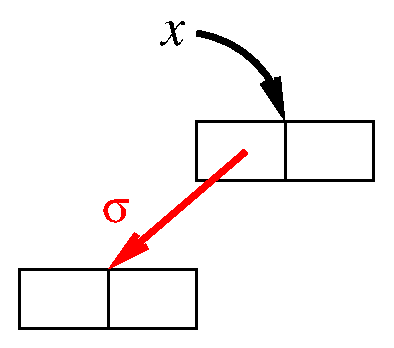
\epsfig{file=live-analysis1.eps, height=2cm}}
%%       \scalebox{.65}{
%%           \psset{unit=1mm}
%%           \psset{linewidth=.5mm}
%%           \begin{pspicture}(0,0)(90,0)
%%             %%%%%%%%%%%%%%%%%%%%%%%%%%%%%%%%%%%%%%%%%%%%%%%%%%%%%%%%%%%%%%%%
%%             \putnode{x}{origin}{13}{-10}{\TwoCells{x0}{x1}}
%%             \putnode{startx}{x}{0}{-3}{}
%%             \putnode{after0}{x}{-5}{-30}{}
%%             \putnode{result}{origin}{32}{10}{\TwoCells{resultx}{resulty}}
%%             \putnode{labx}{x}{-7}{10}{\large $(\CAR\ x)$\;{\red $\sigma$} }
%%             \putnode{labr}{result}{-12}{12}{\large $x$}
            
%%             \onslide<1>{\nccurve[nodesepB=-.2,nodesepA=.5,angleA=295,angleB=135]{->}{labr}{result}}
%%             \onslide<2>{\nccurve[nodesepB=-.2,nodesepA=.5,angleA=295,angleB=135,linecolor=red]{->}{labr}{result}}
%%             \nccurve[nodesepB=-.2,angleA=295,angleB=135]{->}{labx}{x}
%%             \onslide<1>{\nccurve[nodesepB=-.2,angleA=270,angleB=75]{*->}{resultx}{x} \bput(.5){\large \acar}}
%%             \onslide<2>{\nccurve[nodesepB=-.2,angleA=270,angleB=75,linecolor=red]{*->}{resultx}{x} \bput(.5){\large \acar}}
%%             \onslide<2>{\nccurve[nodesepB=-.2,angleA=270,angleB=75,
%%                 linestyle=dashed,linecolor=red]{*->}{startx}{after0}
%%               \bput(.5){\large $\alpha$}}
%%           \end{pspicture}
%%       }
%%     \end{column}
%%     \begin{column}{0.65\textwidth}
%%       $\Lapp{{\red{(\CAR \;x)}}}{\sigma} = \{x.\epsilon, \; x.\acar\sigma\}$
%%     \end{column}
%%   \end{columns}
%%   \pause
%%   \bigskip
%%   \bigskip
%%   \bigskip
%% }
%% \only<3->{ 
%%   \begin{columns}[c]
%%     \begin{column}[T]{0.35\textwidth}
%%       %\centerline{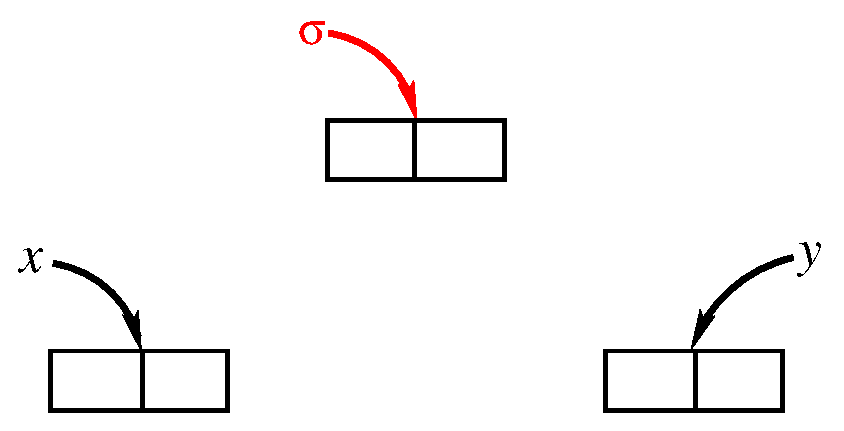
\epsfig{file=live-analysis2.eps, height=2.5cm}}
%%     \end{column}
%%     \begin{column}[T]{0.65\textwidth}
%%       \begin{minipage}{\textwidth}
%%         \begin{eqnarray*}
%%           \Lapp{{\red{(\CONS \;x \;y)}}}{\sigma} &=&  \{x.\alpha \mid \acar\alpha \in \sigma\} \; \cup\\
%%           & &  \{y.\beta \mid \acdr\beta \in \sigma\}
%%         \end{eqnarray*}
        
%%         \onslide<5->{
%%           \begin{itemize}
%%           \item 
%%             \bcar\ -- Removal of a leading \acar
%%             \\
%%             \bcdr\  -- Removal of a leading \acdr
            
%%           \end{itemize}
%%           \begin{eqnarray*}
%%             \Lapp{{\red{(\CONS \;x \;y)}}}{\sigma} &=&  x.\bcar\sigma \cup  y.\bcdr\sigma
%%         \end{eqnarray*}}
%%       \end{minipage}
%%     \end{column}
%%   \end{columns}

%% \raisebox{25mm}{\scalebox{.65}{
%%     \psset{unit=1mm}
%%     \psset{linewidth=.5mm}
%%     \begin{pspicture}(0,0)(90,0)
%%       %%%%%%%%%%%%%%%%%%%%%%%%%%%%%%%%%%%%%%%%%%%%%%%%%%%%%%%%%%%%%%%%
%%       \putnode{x}{origin}{-3}{40}{\TwoCells{x0}{x1}}
%%       \putnode{y}{x}{51}{0}{\TwoCells{y0}{y1}}
%%       \putnode{startx}{x}{0}{-3}{}
%%       \putnode{starty}{y}{0}{-3}{}
%%       \putnode{after0}{x}{-5}{-30}{}
%%       \putnode{after1}{y}{5}{-30}{}
%%       \putnode{result}{origin}{22}{60}{\TwoCells{resultx}{resulty}}
%%       \putnode{labx}{x}{-7}{10}{\large $x$}
%%       \putnode{laby}{y}{7}{10}{\large $y$}
%%       \putnode{labr}{result}{-12}{12}{\large $(\CONS\ x\ y)$\; {\red $\sigma$} }

%%       \nccurve[nodesepB=-.2,angleA=295,angleB=135]{->}{labr}{result}
%%       \nccurve[nodesepB=-.2,angleA=295,angleB=135]{->}{labx}{x}
%%       \nccurve[nodesepB=-.2,angleA=270,angleB=45]{->}{laby}{y}
%%       \nccurve[nodesepB=-.2,angleA=270,angleB=75]{*->}{resultx}{x}
%%       \onslide<4->{        \bput(.5){\large \acar}}
%%       \nccurve[nodesepB=-.2,angleA=270,angleB=105]{*->}{resulty}{y}
%%       \onslide<4->{        \aput(.5){\large \acdr}}
%%       \onslide<4->{\nccurve[nodesepB=-.2,angleA=270,angleB=75,
%%           linestyle=dashed]{*->}{startx}{after0}
%%         \bput(.5){\large $\alpha$}
%% 	\nccurve[nodesepB=-.2,angleA=270,angleB=105,
%%           linestyle=dashed]{*->}{starty}{after1}
%%         \aput(.5){\large ${\mathbf \beta}$}}
%%     \end{pspicture}
%% }}}
%% \end{frame}
%% %%%%%%%%%%%%%%%%%%%%%%%%%%%%%%%%%%%%%%%%%%%%%%%%%%%%%%
%% %%%%%%%%%%%%%%%%%%%%%%%%%%%%%%%%%%%%%%%%%%%%%%%%%%%%%%
%% \begin{frame}{Liveness Analysis of User Defined Functions}
%%   \setbeamercovered{transparent}
%%   \begin{columns}[c]
 \begin{column}[T]{0.4\textwidth}
\hspace*{-.3cm}\renewcommand{\arraystretch}{1}{
	  \begin{uprogram}
	    \UNL{1}\hspace*{-.4cm} $\pi_\mainpgm\!\!:\, $(\LET\  \px\  $\leftarrow$ ($\CONS$ ($+$ 5 2) \NIL)  \IN
            \UNL{2}   \hspace*{-.3cm}   $\pi_9\!\!:\, $(\LET\ \pz\ $\leftarrow$ ($\CONS$ ($+$ 4 5 ) \px) \IN
	    \UNL{3}   \hspace*{-.3cm}   $\pi_9\!\!:\, $(\SIF\ $*$
            \UNL{4}   \hspace*{-.35cm} $\pi_{10}\!\!:\, $(\LET\ \pw\  $\leftarrow$  (\plength\ \pz) \IN
            \UNL{5}   \hspace*{-.38cm}  $\pi_{11}\!\!:\, $(\RETURN\ \pw) 
	    \UNL{4}   \hspace*{-.35cm}  $\pi_{12}\!\!:\, $(\LET\ \pb\  $\leftarrow$ (\pfun\  \pz) \IN
            \UNL{5}   \hspace*{-.38cm} $\pi_{13}\!\!:\,$(\RETURN\ \pb))))))
\end{uprogram}}
 \end{column}
 \begin{column}[T]{0.68\textwidth}
\hspace*{.4cm}  \renewcommand{\arraystretch}{1}{
  \begin{uprogram}
    \UNL{1} (\DEFINE\ (\plength~\lista)

    \UNL{2}  $\pi_1\!\!:\, $(\LET\ \xtest\ $\leftarrow $\ (\NULLQ~\lista) \IN


    \UNL{3}     $\pi_2\!\!:\, $(\SIF\ \xtest

~$\pi_3\!\!:$(\RETURN\ $0$) 
 
          \UNL{4} \hspace*{-.05cm}    
 $\pi_4\!\!:\, $(\LET\ \xtl\  $\leftarrow$\   (\CDR\ \lista) \IN

	  \UNL{5}  \hspace*{-.05cm}
          $\pi_5\!\!:\,$(\LET\ \xrec\  $\leftarrow$ (\plength\ \ \xtl\ ) \IN


          \UNL{6} \hspace*{-.05cm}   $\pi_6\!\!:\, $(\LET\ \xhd\  $\leftarrow$  $1$)  \IN


          \UNL{7}  \hspace*{-.05cm}   $\pi_7\!\!:\,$(\LET\ \xans\  $\leftarrow$ ($+$\ \ \xhd\ \ \xrec)  \IN 

          \UNL{8} \hspace*{-.05cm}
$\pi_8\!\!:\, $ (\RETURN\ \xans)))))))
\end{uprogram}}
 \end{column}
\end{columns}

%%   \begin{itemize}
%%   \item Compute liveness of \pz\ at $\pi_{10}$.
%%   \item Get context independent summary of \plength\ ($\Lf{\plength}{1}{\sigma}$).
%%   \end{itemize}
%%   Key Observation : Liveness of function arguments will always be in terms of the
%%   input demand $\sigma$
%%   \setbeamercovered{invisible}
%%   \raisebox{-25mm}{\scalebox{.85}{
%%       %%%%%%%%%%%%%%%%%%%%%Uday's stuff%%%%%%%%%%%%%%%%%%%%%%%%%
%%       \psset{unit=1mm}
%%       \psset{linewidth=.3mm}
%%       \begin{pspicture}(0,0)(180,30)
%%         %\psgrid[xunit=1cm,yunit=1cm,gridwidth=.2pt,subgridwidth=.1pt,subgriddiv=5,subgridcolor=gray,gridcolor=blue](0,0)(18,10)
%% 	%\psframe(0,0)(73,60)
%% 	%%%%%%%%%%%%%%%%%%%%%%%%%%%%%%%%%%%%%%%%%%%%%%%%%%%%%%%%%%%%%%%%
%% 	%% \onslide<1-5>{\putnode{o}{origin}{26}{72}{\large\red $\sigma_{\xmain} =
%%         %%     \sigma{_{all}}$}}
%% 	\putnode{call1}{origin}{102}{100}{\large\red $\{\epsilon\}$}
%% 	\putnode{appendentry}{origin}{94}{106}{\large\red
%%             $\Lf{\plength}{1}{\sigma} =$}
%%         \putnode{sigma1}{appendentry}{16}{0}{\large\red $\sigma_1$}
%%         \putnode{un}{sigma1}{4}{0}{\large\red $\cup$} 
%% 	\nccurve[nodesepB=-.2,angleA=-11,angleB=-107,linecolor=red]{->}{call1}{sigma1}
%% 	\putnode{call2}{origin}{109}{88}{\large\red $\acdr\Lf{\plength}{1}{\epsilon}$}
%%           \putnode{sigma2}{un}{4}{0}{\large\red $\sigma_2$}
%%         \nccurve[nodesepB=-.2,angleA=25,angleB=-135,linecolor=red]{->}{call2}{sigma2}
%%   \end{pspicture}}}
%% \end{frame}

%% %%%%%%%%%%%%%%%%%%%%%%%%%%%%%%%%%%%%%%%%%%%%%%%%%%%%%%
%% %%%%%%%%%%%%%%%%%%%%%%%%%%%%%%%%%%%%%%%%%%%%%%%%%%%%%%

%% \begin{frame}{Liveness analysis -- Demand Summary}

%% \setbeamercovered{transparent}
%% \small
%% \begin{columns}[c]
%%  \begin{column}[T]{0.45\textwidth}
%%    \hspace*{-.3cm}\renewcommand{\arraystretch}{1}{
%%      \begin{uprogram}
%%        \UNL{1}\hspace*{-.4cm} $\pi_\mainpgm\!\!:\, $(\onslide<0>{\LET\  \px\  $\leftarrow$ ($\CONS$ ($+$ 5 2) \NIL)  \IN}
%%        \UNL{2}   \hspace*{-.3cm}   $\pi_9\!\!:\, $\onslide<0>{(\LET\ \pz\ $\leftarrow$ ($\CONS$ ($+$ 4 5 ) \px) \IN}
%%        \UNL{3}   \hspace*{-.3cm}   $\pi_{10}\!\!:\, $\onslide<0>{(\SIF\ $*$}
%%        \UNL{4}   \hspace*{-.35cm} $\pi_{11}\!\!:\, $\onslide<0>{(\LET\ \pw\  $\leftarrow$  }(\plength\ \pz) \onslide<0>{(\IN}
%%        \UNL{5}   \hspace*{-.38cm}  $\pi_{12}\!\!:\, $\onslide<0>{(\RETURN\ \pw)}
%%        \UNL{4}   \hspace*{-.35cm}  $\pi_{13}\!\!:\, $\onslide<0>{(\LET\ \pb\  $\leftarrow$ (\pfun\  \pz) \IN}
%%        \UNL{5}   \hspace*{-.38cm} $\pi_{14}\!\!:\,$\onslide<0>{(\RETURN\ \pb)))))})
%%    \end{uprogram}}
%%  \end{column}
%%  \begin{column}[T]{0.60\textwidth}
%% \hspace*{.4cm}  \renewcommand{\arraystretch}{1}{
%%   \begin{uprogram}
%%      \UNL{1} (\DEFINE\ (\plength~\lista)

%%     \UNL{2}  $\pi_1\!\!:\, $\onslide<0>{(\LET\ \xtest\ $\leftarrow $\ (\NULLQ~\lista) \IN}


%%     \UNL{3}     $\pi_2\!\!:\, $\onslide<0>{(\SIF\ \xtest}

%% ~$\pi_3\!\!:$\onslide<0>{(\RETURN\ $0$)}
 
%%           \UNL{4} \hspace*{-.05cm}    
%%  $\pi_4\!\!:\, $\onslide<0>{(\LET\ \xtl\  $\leftarrow$\   (\CDR\ \lista) \IN}

%% 	  \UNL{5}  \hspace*{-.05cm}
%%           $\pi_5\!\!:\,$\onslide<0>{(\LET\ \xrec\  $\leftarrow$ }(\plength\ \ \xtl\ ) \onslide<0>{\IN}


%%           \UNL{6} \hspace*{-.05cm}   $\pi_6\!\!:\, $\onslide<0>{(\LET\ \xhd\  $\leftarrow$  $1$)  \IN}


%%           \UNL{7}  \hspace*{-.05cm}   $\pi_7\!\!:\,$\onslide<0>{(\LET\ \xans\  $\leftarrow$ ($+$\ \ \xhd\ \ \xrec)  \IN}

%%           \UNL{8} \hspace*{-.05cm}
%% $\pi_8\!\!:\, $\onslide<0>{(\RETURN\ \xans))))))})
 
%% \end{uprogram}}
%%  \end{column}
%% \end{columns}
%% \setbeamercovered{invisible}
%%       \raisebox{-25mm}{\scalebox{.85}{
%% 	%%%%%%%%%%%%%%%%%%%%%Uday's stuff%%%%%%%%%%%%%%%%%%%%%%%%%
%%       \psset{unit=1mm}
%%       \psset{linewidth=.3mm}
%%       \begin{pspicture}(0,0)(180,30)
%% %\psgrid[xunit=1cm,yunit=1cm,gridwidth=.2pt,subgridwidth=.1pt,subgriddiv=5,subgridcolor=gray,gridcolor=blue](0,0)(18,10)
%% 	%\psframe(0,0)(73,60)
%% 	%%%%%%%%%%%%%%%%%%%%%%%%%%%%%%%%%%%%%%%%%%%%%%%%%%%%%%%%%%%%%%%%
%% 	\putnode{o}{origin}{26}{72}{\large\red $\sigma_{\xmain} =
%%           \sigma{_{all}}$}
%% 	\putnode{call1}{origin}{41}{58}{\large\red $\sigma_1$
%% 	\nccurve[nodesepB=-.2,angleA=270,angleB=135,linecolor=red]{->}{o}{call1}}
%% 	\putnode{appendentry}{origin}{85}{72}{\large\red
%%           $\sigma_{\plength} = \sigma_1 \cup  \sigma_2$}
%% 	\nccurve[nodesepB=-.2,angleA=45,angleB=165,linecolor=red]{->}{call1}{appendentry}
%% 	\putnode{call2}{origin}{125}{52}{\large\red $\sigma_2$}
%% 	\nccurve[nodesepB=-.2,angleA=270,angleB=135,linecolor=red]{->}{appendentry}{call2}
%% 	\nccurve[nodesepB=-.2,angleA=65,angleB=0,linecolor=red]{->}{call2}{appendentry}

%%       \end{pspicture}}}

%% \vspace*{-2cm}
%% \footnotesize
%% \begin{columns}[c]
%%   \begin{column}[T]{0.40\textwidth}
%%     \scriptsize
%%     \centerline{\bf Liveness environments:}
%%     \bigskip
%%     %% $\Lanv{1}{\lista} = \{\epsilon\} \cup  \acar\bcar\sigma_\append\; \cup $\\
%%     %% $\;\;\;\;\;\;\;\;\;\;\;\acdr\Lf{\append}{1}{\bcdr\sigma_{\append}}$\\
%%     %% $\Lanv{1}{\listb} = \sigma \cup \Lf{\append}{2}{\bcdr\sigma_{\append}}$\\
%%     %% \ldots\\
%%     %% $\Lanv{9}{\py}  = $ \Lf{\append}{1}{\{\epsilon,
%%     %%   \acdr\} \cup \acdr\acar\sigma_{\mathit{\!all}}} \\
%%   \end{column}
%%   \begin{column}[T]{0.30\textwidth}
%%     \scriptsize
%%     \centerline{\bf Demand summaries:}
    
%%     \begin{align*}
%%       &\sigma_{\xmain} = \sigma_{all}\\
%%       &\sigma_{\plength} = \sigma_{all} \cup\  \{\epsilon\}
%%     \end{align*}
    
%%   \end{column}
%%   \begin{column}[T]{0.38\textwidth}
%%     \scriptsize
%%     \centerline{\bf Function summaries:}
%%     \bigskip
%%     $\Lf{\plength}{1}{\sigma} = \{\epsilon\} \cup \acdr\Lf{\plength}{1}{\epsilon}$
%%   \end{column}
%% \end{columns}
%% \end{frame}
%%%%%%%%%%%%%%%%%%%%%%%%%%%%%%%%%%%%%%%%%%%%%%%%%%%%%%
\begin{frame}[t]{Summary of Analysis Results}
  \scriptsize
  \begin{columns}[c]
    \begin{column}[T]{0.33\textwidth}
      \vspace*{1.5cm}
      \centerline{\bf Liveness at program points:}
      \begin{align*}
        \Lanv{9}{\px}  &=  \bcdr\Lf{\plength}{1}{\sigma_{\mathit{\!all}}} \\
        \;\;\;\;\;\;\;\;\;\;  &\cup\; \bcdr\Lf{\pfun}{1}{\sigma_{\mathit{\!all}}}\\ 
      \end{align*}
    \end{column}
    \begin{column}[T]{0.33\textwidth}
      \vspace*{1.5cm}
      \centerline{\bf Demand summaries:}
      \begin{align*}
        &\sigma_{\xmain} = \sigma_{all}\\
        &\sigma_{\plength} = \sigma_{all} \cup \{\epsilon\}\\
        &\sigma_{\pfun} = \sigma_{all}\\
      \end{align*}
    \end{column}
    
    \begin{column}[T]{0.33\textwidth}
      \vspace*{1.5cm}
      \centerline{\bf Function summaries:}
      \begin{align*}
        &\Lf{\plength}{1}{\sigma} = \{\epsilon\} \cup \acdr\Lf{\plength}{1}{\epsilon}\\
        &\Lf{\pfun}{1}{\sigma} = \{\epsilon\} \cup \{\acar\sigma\}\\
      \end{align*}
    \end{column}
  \end{columns}
\end{frame}

%%%%%%%%%%%%%%%%%%%%%%%%%%%%%%%%%%%%%%%%%%%%%%%%%%%%%%
\begin{frame} {Handling possible non-evaluation}
  \begin{itemize}
  \item Liveness no longer remains independent of demand $\sigma$ \\
    \begin{itemize}
    \item If (\CAR~\px) is not evaluated at all, it should not generate any liveness for \px
    \end{itemize}
  \item Require a new terminal \clazy\ with following semantics
    \begin{align*}
      \clazy\sigma \hookrightarrow & \left\{ 
      \begin{array}{ll}
        \emptyset&\mbox{if}~\sigma = \emptyset\\
        \{\epsilon\} & \mbox{otherwise}
      \end{array}\right.\\ & \\
%      \Lapp{(\CAR \;\px)}{\sigma} &= \px.\{\clazy, \acar\}\sigma
    \end{align*}
  \end{itemize}
\end{frame}
%%%%%%%%%%%%%%%%%%%%%%%%%%%%%%%%%%%%%%%%%%%%%%%%%%%%%%
\begin{frame}{Handling lazy semantics: Closures}
\normalsize
  \begin{itemize}\itemsep2em
  \item Laziness complicates liveness analysis itself. 
    \begin{itemize}
    \item Data is made live by evaluation of closures
    \item In lazy languages, the place in the program
      where this evaluation takes place cannot be statically determined
    \end{itemize}
    \pause
  \item Liveness-based garbage collector significantly more complicated than that for an eager language.
    \begin{itemize}
    \item Distinguish between stack variables and closure variables.
    \item Need to track liveness of closure variables.
    \item Solution: carry the liveness information in the closure itself.
    \item For precision: need to update the liveness information as execution progresses.
    \end{itemize}
  \end{itemize}
\end{frame}
%%%%%%%%%%%%%%%%%%%%%%%%%%%%%%%%%%%%%%%%%%%%%%%%%%%%%%
\begin{frame}{Handling lazy semantics: Closures}
  \begin{columns}[c]
    \begin{column}[T]{0.5\textwidth}
      \hspace*{-.3cm}\renewcommand{\arraystretch}{1}{
        \begin{uprogram}
          \UNL{1}\hspace*{-.4cm} $\pi_8\!\!:\, $(\LET\  \px\  $\leftarrow$ ($\CONS$ ($+$ 5 2) \NIL)  \IN
          \UNL{2}   \hspace*{-.3cm}   $\pi_9\!\!:\, $(\LET\ \pz\ $\leftarrow$ ($\CONS$ ($+$ 4 5 ) \px) \IN
          %% \UNL{3}   \hspace*{-.3cm}   $\pi_{10}\!\!:\, $(\SIF\ $*$
          %% \UNL{4}   \hspace*{-.35cm} $\pi_{11}\!\!:\, $(\LET\ \pw\  $\leftarrow$ (\plength\ \pz) (\IN
          %% \UNL{5}   \hspace*{-.38cm}  $\pi_{12}\!\!:\, $(\RETURN\ \pw)
          \UNL{2}   \ldots
          \UNL{2}   \hspace*{-.35cm}  $\pi_{13}\!\!:\, $(\LET\ \pb\  $\leftarrow$ (\CONS\  \pz\ \NIL) \IN
          \UNL{3}   \hspace*{-.38cm} $\pi_{14}\!\!:\,$(\RETURN\ \pb))))))
   \end{uprogram}}
    \end{column}
    \begin{column}[T]{0.5\textwidth}
      \begin{itemize}
      \item \pz\ {\em escapes} from the scope it was created.
      \item During GC, we require program point of use of \pz.
      \item Carry program point of last use in closure.
      \end{itemize}
    \end{column}
  \end{columns}
\end{frame}
%%%%%%%%%%%%%%%%%%%%%%%%%%%%%%%%%%%%%%%%%%%%%%%%%%%%%%
\begin{frame}{Handling lazy semantics: Closures}
\begin{columns}[c]
    \begin{column}[T]{0.5\textwidth}
      \hspace*{-.3cm}\renewcommand{\arraystretch}{1}{
        \begin{uprogram}
          \UNL{1}\hspace*{-.4cm} $\pi_8\!\!:\, $(\LET\  \px\  $\leftarrow$ ($\CONS$ ($+$ 5 2) \NIL)  \IN
          \UNL{2}   \hspace*{-.3cm}   $\pi_9\!\!:\, $(\LET\ \pz\ $\leftarrow$ ($\CONS$ ($+$ 4 5 ) \px) \IN
          \UNL{3}   \hspace*{-.3cm}   $\pi_{10}\!\!:\, $(\SIF\ $*$
          \UNL{4}   \hspace*{-.35cm} $\pi_{11}\!\!:\, $(\LET\ \pw\  $\leftarrow$ (\plength\ \pz) (\IN
          \UNL{5}   \hspace*{-.38cm}  $\pi_{12}\!\!:\, $(\RETURN\ \pw)
          \UNL{4}   \hspace*{-.35cm}  $\pi_{13}\!\!:\, $(\LET\ \pb\  $\leftarrow$ (\pfun\  \pz) \IN
          \UNL{5}   \hspace*{-.38cm} $\pi_{14}\!\!:\,$(\RETURN\ \pb))))))
   \end{uprogram}}
    \end{column}
    \begin{column}[T]{0.5\textwidth}
      \begin{itemize}
      \item \px\ is live at $\pi_{9}$  because of its probable use at $\pi_{13}$
      \item If $*$ evaluates to true, then \px\ is not live.
      \item Update liveness of closure arguments as execution proceeds.
      \end{itemize}
    \end{column}
  \end{columns}  
\end{frame}
%%%%%%%%%%%%%%%%%%%%%%%%%%%%%%%%%%%%%%%%%%%%%%%%%%%%%%
\begin{frame}[t]{Modified Analysis Results}
  \scriptsize
  \begin{columns}[c]
    \begin{column}[T]{0.33\textwidth}
      \vspace*{1.5cm}
      \centerline{\bf Liveness at program points:}
      \begin{align*}
        \Lanv{9}{\px}  &=  \bcdr\Lf{\plength}{1}{\sigma_{\mathit{\!all}}} \\
        \;\;\;\;\;\;\;\;\;\;  &\cup\; \bcdr\Lf{\pfun}{1}{\sigma_{\mathit{\!all}}}\\ 
      \end{align*}
    \end{column}
    \begin{column}[T]{0.33\textwidth}
      \vspace*{1.5cm}
      \centerline{\bf Demand summaries:}
      \begin{align*}
        &\sigma_{\xmain} = \sigma_{all}\\
        &\sigma_{\plength} = \sigma_{all} \cup \{\clazy\sigma_{\plength}\}\\
        &\sigma_{\pfun} = \sigma_{all}\\
      \end{align*}
    \end{column}
    
    \begin{column}[T]{0.33\textwidth}
      \vspace*{1.5cm}
      \centerline{\bf Function summaries:}
      \begin{align*}
        &\Lf{\plength}{1}{\sigma} = \{\clazy\sigma\} \cup \acdr\Lf{\plength}{1}{\clazy\sigma}\\
        &\Lf{\pfun}{1}{\sigma} = \{\clazy\sigma\} \cup \{\acar\sigma\}\\
      \end{align*}
    \end{column}
  \end{columns}
\end{frame}
%%%%%%%%%%%%%%%%%%%%%%%%%%%%%%%%%%%%%%%%%%%%%%%%%%%%%%
%%%%%%%%%%%%%%%%%%%%%%%%%%%%%%%%%%%%%%%%%%%%%%%%%%%%%%

\begin{frame}{Solution of the equations}

  View the equations as grammar rules:
  \scalebox{0.75}{
  \begin{columns}
    \begin{column}[T]{.5\textwidth}
      \begin{eqnarray*}
          \Lf{\plength }{1}{\sigma} &=& \Df{\plength}{1}\sigma\\
          \Df{\plength}{1} &=& \clazy \cup \acdr\Df{\plength}{1}\clazy \\
                                &&\cup\;\;\; \clazy\Df{\plength}{1}{\clazy}\\
          \Lanv{9}{\px}  &=&  \bcdr\Lf{\plength}{1}{\sigma_{\mathit{\!all}}} \\
                           &&  \cup\; \bcdr\Lf{\pfun}{1}{\sigma_{\mathit{\!all}}}
      \end{eqnarray*}
    \end{column}
    \begin{column}[T]{0.5\textwidth}
      \begin{eqnarray*}
        \var{\LfNoSigma{\plength}{1}} &\rightarrow& \var{\Df{\plength}{1}} \\
        \var{\Df{\plength}{1}}   &\rightarrow&   \clazy\var{\Df{\plength}{1}}
        \mid                 \acdr\var{\Df{\plength}{1}}\clazy \\
                            &&\mid\;\; \clazy\var{\Df{\plength}{1}}\clazy\\
        \var{\Lanv{9}{\px}}  &\rightarrow&  \bcdr\var{\LfNoSigma{\plength}{1}} \\
                           &&  \cup\; \bcdr\var{\LfNoSigma{\pfun}{1}}
      \end{eqnarray*}
    \end{column}
  \end{columns}
  }
  \linebreak
  \linebreak
  \linebreak
  The  solution of \Lanv{9}{\px} is the   language  $\mathscr{L}(\Lanv{9}{\px})$ generated    by    it.
\end{frame}

%%%%%%%%%%%%%%%%%%%%%%%%%%%%%%%%%%%%%%%%%%%%%%%%%%%%%%

%%%%%%%%%%%%%%%%%%%%%%%%%%%%%%%%%%%%%%%%%%%%%%%%%%%%%%
\begin{frame}{Working of Liveness-based GC (Mark phase)}
  \begin{itemize}
  \item GC invoked at a program point $\pi$
  \item GC traverses a path $\alpha$ starting from a root variable $x$.
  \item GC consults $\Lanv{\pi}{x}$: 
    \begin{itemize}
    \item Does $\alpha \in \mathscr{L}(\Lanv{\pi}{x})$ ?
    \item If yes, then mark the current cell
    \end{itemize}
    \pause
  \item  Note  that  $\alpha$  is a  {\em  forward}-only  access  path
    \begin{itemize}
    \item consisting  only of  edges \acar\  and \acdr,  but not  \bcar\ or
      \bcdr\ or \clazy
    \item But $\mathscr{L}(\Lanv{\pi}{x})$ has access paths marked with \bcar/\bcdr\ for \acar/\acdr\  removal
  arising from the \CONS\  rule and \clazy\ added to handle lazy evaluation.
    \end{itemize}
  \end{itemize}
\end{frame}

%%%%%%%%%%%%%%%%%%%%%%%%%%%%%%%%%%%%%%%%%%%%%%%%%%%%%%
\begin{frame}{GC decision problem}
\begin{itemize}
\item Deciding the
  membership in  a CFG augmented  with a
  fixed set of unrestricted productions.
  \begin{align*}
    \bcar\acar    \rightarrow    \epsilon\\
    \bcdr\acdr    \rightarrow   \epsilon\\
  \end{align*}
\item We have proven the problem to be undecidable
  \begin{itemize}
  \item Reduction from Halting problem.
  \end{itemize}
\end{itemize}
\end{frame}
%%%%%%%%%%%%%%%%%%%%%%%%%%%%%%%%%%%%%%%%%%%%%%%%%%%%%%
\begin{frame}{Practical \bcar/\bcdr\  simplification}

\begin{itemize}
\item The simplification is possible to do on a finite state automaton.
\item Over-approximate the CFG by an automaton
  (Mohri-Nederhoff transformation).
\item Perform \acar/\acdr\ removal on the automaton.
\item Perform \clazy\ removal.
\end{itemize}

\end{frame}
%%%%%%%%%%%%%%%%%%%%%%%%%%%%%%%%%%%%%%%%%%%%%%%%%%%%%%
%% \begin{frame}{Example}
%%   \scriptsize
%%   \begin{columns}[c]
%%     \begin{column}[T]{.5\textwidth}
%%       {Grammar for \Lanv{9}{\px}}
%%       \begin{eqnarray*}
%%         &&  \Lf{\plength }{1}{\sigma} = \Df{\plength}{1}\sigma,~\mbox{and}\\
%%         &&   \Df{\plength}{1} = \clazy \cup \acdr\Df{\plength}{1}\clazy
%%         \cup \clazy\Df{\plength}{1}{\clazy}
%%       \end{eqnarray*}
%%     \end{column}
%%     \begin{column}[T]{.5\textwidth}
%%       After Mohri-Nederhoff transformation
%%        \begin{eqnarray*}              
%%          \var{\Df{\plength}{1}}   &\rightarrow&   \clazy\varnew{\Df{\plength}{1}}
%%          \mid                 \acdr\var{\Df{\plength}{1}}                 \mid
%%          \clazy\var{\Df{\plength}{1}}\\  \varnew{\Df{\plength}{1}}  &\rightarrow&
%%          \clazy\varnew{\Df{\plength}{1}} \mid \epsilon
%%        \end{eqnarray*}
%%     \end{column}
%%   \end{columns}
%% \end{frame}
%%%%%%%%%%%%%%%%%%%%%%%%%%%%%%%%%%%%%%%%%%%%%%%%%%%%%%

\begin{frame}{Example automaton and its simplification}
\newcommand{\nfaD}{%
  \scalebox{.99}{
    \psset{unit=1mm,nodesep=0mm,labelsep=0.5mm}
    \begin{pspicture}(3,-1)(28,9)%\psgrid
      \putnode{t0}{origin}{-4}{15}{\Lf{\plength}{1}{\sigma}} 
      \putnode{t1}{t0}{20}{0}{\pscirclebox{\mbox{$q_0$}}}
      \hspace{5mm} 
      \putnode{t2}{t1}{15}{0}{\pscirclebox[doubleline=true]{\mbox{$q_1$}}} 
      \psset{arrows=->} \ncline{t0}{t1} 
      \ncline{t1}{t2} 
      \putnode{l0}{t1}{7}{2}{\clazy} 
      \nccurve[angleA=45, angleB=135, ncurv=2, nodesep=-1]{t1}{t1} 
      \putnode{l1}{t1}{0}{6}{\acdr, \clazy} 
      \nccurve[angleA=45,
        angleB=135, ncurv=1.5, nodesep=-1]{t2}{t2} 
      \putnode{l2}{t2}{0}{7}{\clazy}
    \end{pspicture}
}}

\newcommand{\zcarliveness}{%
  \scalebox{.99}{
    \psset{unit=1mm,nodesep=0mm,labelsep=0.5mm}
    \begin{pspicture}(3,-1)(28,9)%\psgrid
      \putnode{t0}{origin}{2}{1}{\mbox{zcar}} 
      \putnode{t1}{t0}{18}{0}{\pscirclebox{\mbox{$q_0$}}}
      \hspace{5mm} 
      \putnode{t2}{t1}{15}{5}{\pscirclebox{\mbox{$q_1$}}} 
      \putnode{t3}{t2}{15}{0}{\pscirclebox[doubleline=true]{\mbox{$q_2$}}} 
      \psset{arrows=->} \ncline{t0}{t1} 
      \ncline{t1}{t2} 
      \ncline{t2}{t3} 
      \putnode{l0}{t1}{7}{5}{\bcar} 
      \putnode{l1}{t2}{7}{2}{\acar}
      \putnode{t4}{t1}{15}{-5}{\pscirclebox[doubleline=true]{\mbox{$q_3$}}}
      \ncline{t1}{t4}
      \putnode{l2}{t1}{7}{0}{\bcar} 
      \nccurve[angleA=-45, angleB=-135, ncurv=1.5, nodesep=-1]{t4}{t4} 
      \putnode{l3}{t4}{0}{-8}{\acdr} 
    \end{pspicture}
}}

\newcommand{\zcarlivenesssimpl}{%
  \scalebox{.99}{
    \psset{unit=1mm,nodesep=0mm,labelsep=0.5mm}
    \begin{pspicture}(3,-1)(28,9)%\psgrid
      \putnode{t0}{origin}{2}{1}{\mbox{zcar}} 
      \putnode{t1}{t0}{18}{0}{\pscirclebox{\mbox{$q_0$}}}
      \hspace{5mm} 
      \putnode{t2}{t1}{15}{5}{\pscirclebox{\mbox{$q_1$}}} 
      \putnode{t3}{t2}{15}{0}{\pscirclebox[doubleline=true]{\mbox{$q_2$}}} 
      \psset{arrows=->} \ncline{t0}{t1} 
      \ncline{t1}{t2} 
      \ncline{t2}{t3}
      \nccurve[angleA=65, angleB=115, ncurv=0.75, nodesep=-1, linecolor=red]{t1}{t3} 
      \putnode{l0}{t1}{7}{5}{\bcar} 
      \putnode{l1}{t2}{7}{2}{\acar}
      \putnode{l2}{t1}{13}{14}{\color{red}$\epsilon$}
      \putnode{t4}{t1}{15}{-5}{\pscirclebox[doubleline=true]{\mbox{$q_3$}}}
      \ncline{t1}{t4}
      \putnode{l3}{t1}{7}{0}{\bcar} 
      \nccurve[angleA=-45, angleB=-135, ncurv=1.5, nodesep=-1]{t4}{t4} 
      \putnode{l3}{t4}{0}{-8}{\acdr} 
    \end{pspicture}
}}

\newcommand{\zcarlivenessfinal}{%
  \scalebox{.99}{
    \psset{unit=1mm,nodesep=0mm,labelsep=0.5mm}
    \begin{pspicture}(3,-1)(28,9)%\psgrid
      \putnode{t0}{origin}{2}{-20}{\mbox{zcar}} 
      \putnode{t1}{t0}{18}{0}{\pscirclebox[doubleline=true]{\mbox{$q_0$}}}
      \psset{arrows=->} \ncline{t0}{t1} 
    \end{pspicture}
}}

\newcommand{\zcdrliveness}{%
  \scalebox{.99}{
    \psset{unit=1mm,nodesep=0mm,labelsep=0.5mm}
    \begin{pspicture}(3,-1)(28,9)%\psgrid
      \putnode{t0}{origin}{-9}{0}{\mbox{\Lanv{9}{\px}}} 
      \putnode{t1}{t0}{18}{0}{\pscirclebox{\mbox{$q_0$}}}
      \hspace{5mm} 
      \putnode{t2}{t1}{15}{5}{\pscirclebox{\mbox{$q_1$}}} 
      \putnode{t3}{t2}{15}{0}{\pscirclebox[doubleline=true]{\mbox{$q_2$}}} 
      \psset{arrows=->} \ncline{t0}{t1} 
      \ncline{t1}{t2} 
      \ncline{t2}{t3} 
      \putnode{l0}{t1}{7}{5}{\bcdr} 
      \putnode{l1}{t2}{7}{2}{\acar}
      \putnode{t4}{t1}{15}{-5}{\pscirclebox[doubleline=true]{\mbox{$q_3$}}}
      \ncline{t1}{t4}
      \putnode{l2}{t1}{7}{0}{\bcdr} 
      \nccurve[angleA=-45, angleB=-135, ncurv=1.5, nodesep=-1]{t4}{t4} 
      \putnode{l3}{t4}{0}{-8}{\acdr} 
    \end{pspicture}
}}

\newcommand{\zcdrlivenesssimpl}{%
  \scalebox{.99}{
    \psset{unit=1mm,nodesep=0mm,labelsep=0.5mm}
    \begin{pspicture}(3,-1)(28,9)%\psgrid
      \putnode{t0}{origin}{-9}{1}{\mbox{\Lanv{9}{\px}}} 
      \putnode{t1}{t0}{18}{0}{\pscirclebox{\mbox{$q_0$}}}
      \hspace{5mm} 
      \putnode{t2}{t1}{15}{5}{\pscirclebox{\mbox{$q_1$}}} 
      \putnode{t3}{t2}{15}{0}{\pscirclebox{\mbox{$q_2$}}} 
      \psset{arrows=->} \ncline{t0}{t1} 
      \ncline{t1}{t2} 
      \ncline{t2}{t3}
      \putnode{l0}{t1}{7}{5}{\bcdr} 
      \putnode{l1}{t2}{7}{2}{\acar}
      
      \putnode{t4}{t1}{15}{-5}{\pscirclebox[doubleline=true]{\mbox{$q_3$}}}
      \ncline{t1}{t4}
      \putnode{l3}{t1}{7}{0}{\bcdr} 
      \nccurve[angleA=-65, angleB=-115, ncurv=0.75, nodesep=-1, linecolor=red]{t1}{t4} 
      \nccurve[angleA=-45, angleB=-115, ncurv=1.5, nodesep=-1]{t4}{t4} 
      \putnode{l2}{t1}{8}{-12}{\color{red}$\epsilon$}
      \putnode{l3}{t4}{0}{-8}{\acdr} 
    \end{pspicture}
}}

\newcommand{\zcdrlivenessfinal}{%
  \scalebox{.99}{
    \psset{unit=1mm,nodesep=0mm,labelsep=0.5mm}
    \begin{pspicture}(3,-1)(28,9)%\psgrid
      \putnode{t0}{origin}{10}{-10}{\mbox{\Lanv{9}{\px}}} 
      \putnode{t1}{t0}{18}{0}{\pscirclebox[doubleline=true]{\mbox{$q_0$}}}
      \psset{arrows=->} \ncline{t0}{t1} 
      \nccurve[angleA=-45, angleB=-115, ncurv=1.5, nodesep=-1]{t1}{t1}
      \putnode{l0}{t1}{0}{-7}{\acdr}
    \end{pspicture}
}}



\newcommand{\nfaDF}{%
  \scalebox{.99}{
    \psset{unit=1mm,nodesep=0mm,labelsep=0.5mm}
    \begin{pspicture}(3,-1)(28,9)%\psgrid
      \putnode{t0}{origin}{2}{15}{\Lf{\plength}{1}{\sigma}} 
      \putnode{t1}{t0}{20}{0}{\pscirclebox[doubleline=true]{\mbox{$q_0$}}}
      \hspace{5mm} 
      \putnode{t2}{t1}{15}{0}{\pscirclebox[doubleline=true]{\mbox{$q_1$}}} 
      \psset{arrows=->} \ncline{t0}{t1} 
      \ncline{t1}{t2} 
      \putnode{l0}{t1}{7}{2}{\clazy} 
      \nccurve[angleA=45, angleB=135, ncurv=1.5, nodesep=-1]{t1}{t1} 
      \putnode{l1}{t1}{0}{7}{\acdr, \clazy} 
      \nccurve[angleA=45, angleB=135, ncurv=1.5, nodesep=-1]{t2}{t2} 
      \putnode{l2}{t2}{0}{7}{\clazy}
    \end{pspicture}
}}
\newcommand{\dfaD}{%
  \scalebox{.99}{
    \psset{unit=1mm,nodesep=0mm,labelsep=0.5mm}
    \begin{pspicture}(2,-1)(13,9)
      \putnode{t0}{origin}{1}{10}{\Lf{\plength}{1}{\sigma}}
      \putnode{t1}{t0}{20}{0}{\pscirclebox[doubleline=true]{\mbox{$q_0$}}}     
      \psset{arrows=->}    
      \ncline{t0}{t1}     
      \nccurve[angleA=45, angleB=135, ncurv=1.5, nodesep=-1]{t1}{t1} 
      \putnode{l1}{t1}{0}{7}{\acdr}
    \end{pspicture}
}}


\begin{figure}[t]
\begin{center}
{\scalebox{1.00}{
    \begin{tabular}[T]{c c c}
      \nfaD && \nfaDF \\ & \dfaD & \\
      \zcdrliveness & & \zcdrlivenesssimpl \\ &
      \zcdrlivenessfinal &
    \end{tabular}
}}
\end{center}
\end{figure}

\end{frame}

%%%%%%%%%%%%%%%%%%%%%%%%%%%%%%%%%%%%%%%%%%%%%%%%%%%%%%
\begin{frame}{LGC for a \CONS\ cell}
      \begin{itemize}
      \item Find corresponding automaton for root variable.
      \item If automaton accepts $\epsilon$, copy current cell to live buffer.
      \item Recursively copy the $\CDR$ part with the automaton starting from the state on a $\acdr$ from the current state.
      \newcommand{\lgccons}{}%
\scalebox{.99}{ 
\psset{xunit=.6mm, yunit=.8mm}
\psset{linewidth=.3mm}
\begin{pspicture}(0,15)(150,-45)
% \psframe(0,15)(150,-45)
  %%%%%%%%%%%%%%%%%%%%%%%%%%%%%%%%%%%%%%%%%%%%%%%%%%%%%%%%%%%%%%%%
  \putnode{o}{origin}{13}{-10}{\TwoCells{o1}{o2}}
  \putnode{a}{o}{-15}{-15}{\psframebox{\mbox{ }}}
  \putnode{b}{a}{+30}{0}{\TwoCells{b1}{b2}}
  \nccurve[angleA=-90,angleB=90]{*->}{o1}{a}
  \Aput[.1pt]{\acar}
  \putnode{y}{o}{-10}{12}{\psframebox[linestyle=none,framesep=.5pt]{$\px$}}
  \nccurve[angleA=-90,angleB=90,nodesepB=-.1pt]{*->}{o2}{b}
  \Aput[.1pt]{\acdr}
  \nccurve[angleA=-45,angleB=120]{->}{y}{o}
  \putnode{xa}{b}{-15}{-15}{\mbox{}}
  \nccurve[angleA=-90,angleB=90]{*->}{b1}{xa}
  \Aput[.1pt]{\acar}
  \putnode{xb}{b}{+15}{-15}{\mbox{}}
  \nccurve[angleA=-90,angleB=90]{*->}{b2}{xb}
  \Aput[.1pt]{\acdr}
  %%%%%%%%%%%%%%%%%%%%%%%%%%%%%%%%%%%%%%%%%%%%%%%%%%%%%%
  \putnode{t0}{y}{40}{0}{\Lanv{\pi}{\px}}
  \putnode{t1}{t0}{20}{0}{\pscirclebox[doubleline=true]{\mbox{$q_0$}}}     
  \putnode{t2}{t1}{30}{0}{\pscirclebox[doubleline=true]{\mbox{$q_1$}}}     
  \putnode{t3}{t2}{40}{0}{\pscirclebox[doubleline=true]{\mbox{$q_n$}}}     
  \psset{arrows=->}    
  \ncline[nodesep=0]{t0}{t1}
  \ncline[nodesep=0]{t1}{t2} 
  \Aput[0.1]{\acdr}
  %      \nccoil[angleA=45, angleB=135, ncurv=1.5, nodesep=-1]{t2}{t3} 
  \nczigzag[nodesep=0.1,coilwidth=4mm,coilheight=.3,coilarm=2mm]{t2}{t3} 
  %%%%%%%%%%%%%%%%%%%%%%%%%%%%%%%%%%%%%%%%%%%%%%%%%%%%%%
  \nccurve[nodesep=0.1,linestyle=dashed,angleA=0,angleB=-120]{o}{t1}
  \nccurve[nodesep=0.1, linestyle=dashed,angleA=0,angleB=-105]{b}{t2}
\end{pspicture}
}
\lgccons

      \end{itemize}
\end{frame}

\begin{frame}{LGC for closures}
      \begin{itemize}
      \item Find corresponding automaton for root variable.
      \item If automaton accepts $\epsilon$, copy current cell to live buffer.
      \item For each argument of the closure, use corresponding automaton stored in the closure and copy.
      \scalebox{.99}{ 
\psset{xunit=.6mm, yunit=.8mm}
\psset{linewidth=.3mm}
\begin{pspicture}(0,15)(150,-45)
% \psframe(0,15)(150,-45)
  %%%%%%%%%%%%%%%%%%%%%%%%%%%%%%%%%%%%%%%%%%%%%%%%%%%%%%%%%%%%%%%%
  \putnode{o}{origin}{13}{-10}{\TwoCells{o1}{o2}}
  \putnode{a}{o}{-15}{-15}{\psframebox{\mbox{\ }}}
  \putnode{b}{o}{0}{-5}{\TwoCells{b1}{b2}}
  \nccurve[angleA=-90,angleB=90]{*->}{o1}{a}
  %  \Aput[.1pt]{\acar}
  \putnode{y}{o}{-10}{12}{\psframebox[linestyle=none,framesep=.5pt]{$\px$}}
  % \nccurve[angleA=-90,angleB=90,nodesepB=-.1pt]{*->}{o2}{b}
  % \Aput[.1pt]{\acdr}
  \nccurve[angleA=-45,angleB=120]{->}{y}{o}
  \putnode{xa}{b}{15}{-15}{\psframebox{\mbox{\ }}}
  \nccurve[angleA=-90,angleB=90]{*->}{b1}{xa}
  %  \Aput[.1pt]{\acar}
  %\putnode{xb}{b}{+15}{-15}{\mbox{}}
  % \nccurve[angleA=-90,angleB=90]{*->}{b2}{xb}
  %  \Aput[.1pt]{\acdr}
  %%%%%%%%%%%%%%%%%%%%%%%%%%%%%%%%%%%%%%%%%%%%%%%%%%%%%%
  \putnode{t0}{y}{40}{0}{\Lanv{\pi}{\px}}
  \putnode{t1}{t0}{20}{0}{\pscirclebox[doubleline=true]{\mbox{\ }}}     
  \putnode{t3}{t1}{40}{0}{\pscirclebox[doubleline=true]{\mbox{\ }}}     
  \psset{arrows=->}    
  \ncline[nodesep=0]{t0}{t1}
  %      \nccoil[angleA=45, angleB=135, ncurv=1.5, nodesep=-1]{t2}{t3} 
  \nczigzag[nodesep=0.1,coilwidth=4mm,coilheight=.3,coilarm=2mm]{t1}{t3} 
  %%%%%%%%%%%%%%%%%%%%%%%%%%%%%%%%%%%%%%%%%%%%%%%%%%%%%%


  \putnode{xt0}{y}{40}{-15}{\mbox{\ }}
  \putnode{xt1}{xt0}{20}{0}{\pscirclebox{\mbox{\ }}}
  \putnode{xt3}{xt1}{40}{0}{\pscirclebox[doubleline=true]{\mbox{\ }}}     
  \psset{arrows=->}    
  \ncline[nodesep=0]{xt0}{xt1}
  %      \nccoil[angleA=45, angleB=135, ncurv=1.5, nodesep=-1]{t2}{t3} 
  \nczigzag[nodesep=0.1,coilwidth=4mm,coilheight=.3,coilarm=2mm]{xt1}{xt3} 
  %%%%%%%%%%%%%%%%%%%%%%%%%%%%%%%%%%%%%%%%%%%%%%%%%%%%%%
  \nccurve[nodesep=0.1,linestyle=dashed,angleA=0,angleB=120]{o}{xt1}

  \putnode{zt0}{y}{40}{-30}{\mbox{\ }}
  \putnode{zt1}{zt0}{20}{0}{\pscirclebox{\mbox{\ }}}     
  \putnode{zt3}{zt1}{40}{0}{\pscirclebox[doubleline=true]{\mbox{\ }}}     
  \psset{arrows=->}    
  \ncline[nodesep=0]{zt0}{zt1}
  %      \nccoil[angleA=45, angleB=135, ncurv=1.5, nodesep=-1]{t2}{t3} 
  \nczigzag[nodesep=0.1,coilwidth=4mm,coilheight=.3,coilarm=2mm]{zt1}{zt3} 
  %%%%%%%%%%%%%%%%%%%%%%%%%%%%%%%%%%%%%%%%%%%%%%%%%%%%%%
  \nccurve[nodesep=0.1,linestyle=dashed,angleA=0,angleB=120]{b}{zt1}


\end{pspicture}
}


      \end{itemize}
\end{frame}

%%%%%%%%%%%%%%%%%%%%%%%%%%%%%%%%%%%%%%%%%%%%%%%%%%%%%%
\section{\scshape Results}
\begin{frame}{Experimental Setup}
  \begin{itemize}\itemsep1em
  \item A prototype consisting of:
    \begin{itemize}
    \item An ANF-scheme interpreter
    \item Liveness analyzer
    \item A single-generation copying collector.
     \end{itemize}
  \item The collector optionally uses liveness
    \begin{itemize}
    \item Marks a link during GC only if it is live.
    \end{itemize}
  \item Benchmark programs are mostly from the no-fib suite. 
  \end{itemize}

\end{frame}

%%%%%%%%%%%%%%%%%%%%%%%%%%%%%%%%%%%%%%%%%%%%%%%%%%%%%%
\begin{frame}[t]{GC Results}
\begin{tabular}{|@{\ }c@{\ }|@{\ }r@{\ }|@{\ }r@{\ }|@{\ }r@{\ }|@{\ }r@{\ }|@{\ }r@{\ }|@{\ }r@{\ }|@{\ }r@{\ }|@{\ }r@{\ }@{\ }|@{\ }@{\ }r@{\ }|@{\ }r@{\ }|@{\ }r@{\ }|@{\ }r@{\ }|@{\ }r@{\ }|}
\hline
  & \multicolumn{2}{@{}c@{}|}{DFA}
  & \multicolumn{2}{@{}c@{}|}{\# Collected} 
  & \multicolumn{2}{@{}c@{}|}{\# Touched}
  & \multicolumn{2}{@{}c@{}|}{} 
  & \multicolumn{2}{@{}c@{}|}{}
  & \multicolumn{2}{@{}c@{}|}{GC time}
  &  \\ \cline{2-3}
  &   \# & Generation
  &   \multicolumn{2}{@{}c@{}|}{cells per GC}
  &   \multicolumn{2}{@{}c@{}|}{cells per GC}
  &   \multicolumn{2}{@{}c@{}|}{\#GCs}
  &   \multicolumn{2}{@{}c@{}|}{Drag Reduction (\%)}
  &   \multicolumn{2}{@{}c@{}|}{(sec)} &Speedup \\
\cline{4-13}
{Program}&States&Time (sec) &RGC&LGC&RGC&LGC&RGC&LGC&\#Cells&Time&RGC&LGC&RGC/LGC \\
\hline
\hline

\verb@lambda@ & 3312 & 14.7 & 7271.7 & 7517.1 & 13194.2 & 95644.2 & 775 & 750 & 25.60 & 0.71 & 0.16 & 0.94 & 0.17
\\ \hline

\verb@nperm@ & 2055 & 1.1 & 4684.4 & 8633.2 & 22744.2 & 18808.5 & 710 & 386 & 87.96 & 102.07 & 0.23 & 0.14 & 1.62
\\ \hline

\verb@treejoin@ & 2332 & 2690.5 & 50284.2 & 72317.5 & 1566250.0 & 1553000.0 & 116 & 81 & 12.60 & 1.29 & 3.80 & 3.78 & 1.00
\\ \hline

\verb@lcss@ & 2340 & 13.3 & 8064.7 & 10103.6 & 14177.9 & 12542.8 & 30 & 24 & 1.99 & 1.10 & 0.01 & 0.01 & 0.83
\\ \hline

\verb@sudoku@ & 5672 & 798.5 & 983.9 & 1048.8 & 3091.0 & 5650.9 & 169 & 159 & 8.45 & -0.98 & 0.01 & 0.02 & 0.32
\\ \hline

\verb@fibheap@ & 2254 & 49.8 & 4610.8 & 4736.6 & 33389.9 & 35890.1 & 1002 & 975 & 1.25 & 1.49 & 1.07 & 5.08 & 0.21
\\ \hline

\verb@nqueens@ & 1229 & 0.5 & 17048.1 & 21993.1 & 5680.9 & 985.9 & 511 & 396 & 38.52 & 36.29 & 0.05 & 0.02 & 2.08
\\ \hline

\verb@knightstour@ & 1742 & 5.1 & 229973.0 & 289223.0 & 450027.0 & 454813.0 & 412 & 328 & 5.99 & 1.38 & 4.40 & 8.77 & 0.50
\\ \hline

\verb@gc_bench@ & 729 & 0.1 & 21080.6 & 204817.0 & 183769.0 & 33.0 & 34 & 4 & 660783.87 & 1738598.92 & 0.11 & 0.00 & 0.00
\\ \hline

\end{tabular}
  
\end{frame}
%%%%%%%%%%%%%%%%%%%%%%%%%%%%%%%%%%%%%%%%%%%%%%%%%%%%%%
%******
\section{\scshape Future Work  \& Conclusions} 
\begin{frame}{Scope for future work}
\normalsize
\begin{itemize}\itemsep2em
\item<1-> Reducing GC-time.
  \begin{itemize}
  \item Reducing re-visits to heap nodes.
  \item Hybrid GC (RGC + LGC)
  \end{itemize}
\item<2-> Increasing the scope of the method.
  \begin{itemize}
   \item Higher order functions.
    \begin{itemize}
    \item Specialize all higher order functions (Firstification)
    \item Analysis on the firstified program 
    \item For partial applications, carry information about the {\em base} function
    \end{itemize}
  \end{itemize}
\end{itemize}
\end{frame}

%%%%%%%%%%%%%%%%%%%%%%%%%%%%%%%%%%%%%%%%%%%%%%%%%%%%%%
\begin{frame}{Conclusions}
  \begin{itemize}\itemsep1em
  \item Current garbage collectors leave a lot of memory that can be safely collected. 
  \item By storing extra information in the cell, our method collects dead cells from inside closures also.
  \item By updating liveness information of closures at run-time, we were able to improve precision of GC.
  \item Not covered in this talk:
    \begin{itemize}
    \item The soundness of liveness analysis.
    \item Details of undecidability proof.
    \end{itemize}
    \item Unfinished agenda:
      \begin{itemize}
      \item Improving GC time for a larger fraction of programs.
      \item Extending scope of the method.
    \end{itemize}
  \end{itemize}
\end{frame}
\end{document}
